%!TEX root = ../MainBody.tex

%第四章
\chapter{总体设计}

\section{系统总体结构设计}
\cref{all_module_design}是系统总体结构设计。左边是服务器端,暴露 Restful 服务接口,响应客户端的 HTTP 请求,
返回 Json 数据。右边是 Android 客户端,发起 HTTP 请求,将得到的请求结果保存在本地 Sqlite 数据库中。

\begin{figure}[h]
	\centering
	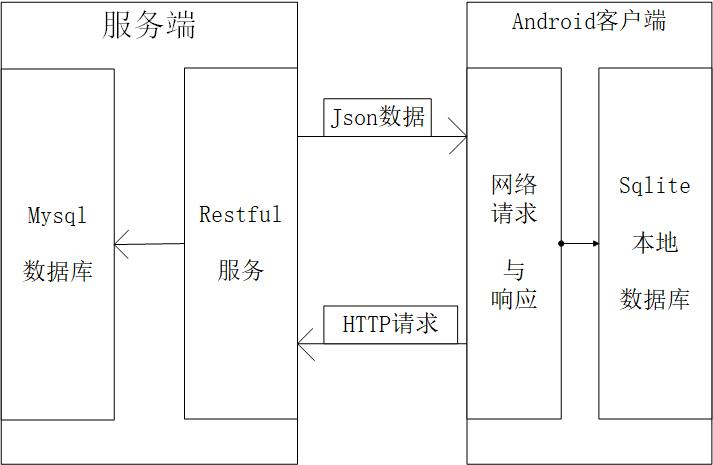
\includegraphics[scale=0.5]{Chapters/UML/system_structrue.jpg}
	\caption{系统总体结构设计}
	\label{all_module_design}
\end{figure}

\begin{figure}[h]
	\centering
	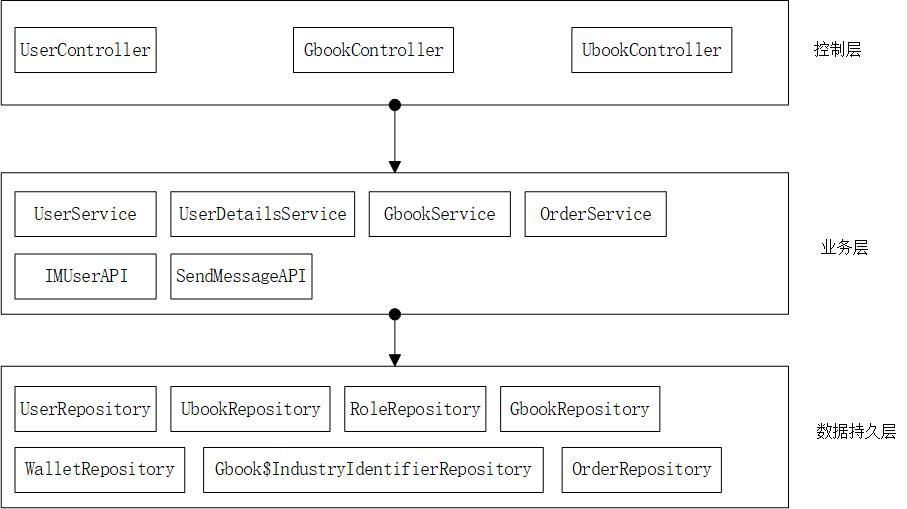
\includegraphics[scale=0.6]{Chapters/UML/system_level_design.jpg}
	\caption{服务端系统分层设计}
	\label{system_level_design}
\end{figure}

\section{服务端系统分层设计}
\cref{system_level_design}是服务端系统分层设计。项目结构分为控制层,业务层和数据持久层。控制层负责响应用户
请求,调用业务层完成请求。业务层进行相关处理,并调用数据持久化层方法完成业务逻辑。数据持久层专一负责数据的存储与
查询等操作。

\section{系统业务流程}

\cref{user_login}是用户登录流程图。用户在客户端输入用户名和密码,将参数上传至应用服务器,服务器首先
判断账户是否存在,然后判断密码是否一致,如果通过判断,则生成 token,并返回给客户端。客户端拿到 token,算作
成功的一次登录。

\begin{figure}[h]
	\centering
	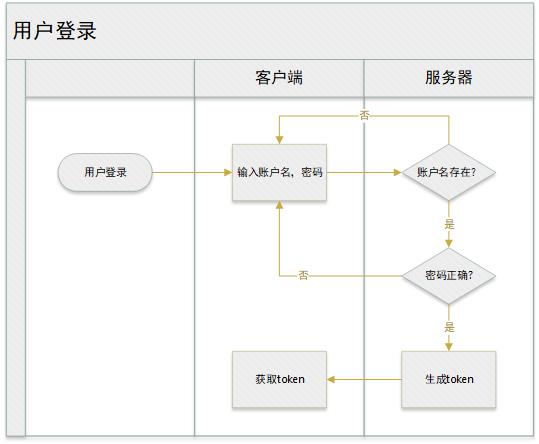
\includegraphics[scale=1]{Chapters/UML/user_login.jpg}
	\caption{用户登录流程图}
	\label{user_login}
\end{figure}

\cref{user_register}是用户注册流程图。用户在客户端输入帐户名,异步发送给应用服务器,服务器判断账户名是否已
存在,如果不可用,则返回错误信息;然后用户输入邮箱,同样异步发送到应用服务器判断是否可用;之后用户在客户端
输入密码和二次密码,两次密码不仅要一致,而且要在客户端判断是否符合密码强度;上述都通过后,请求服务器;服务器
创建账户并返回信息。
	
\begin{figure}[h]
	\centering
	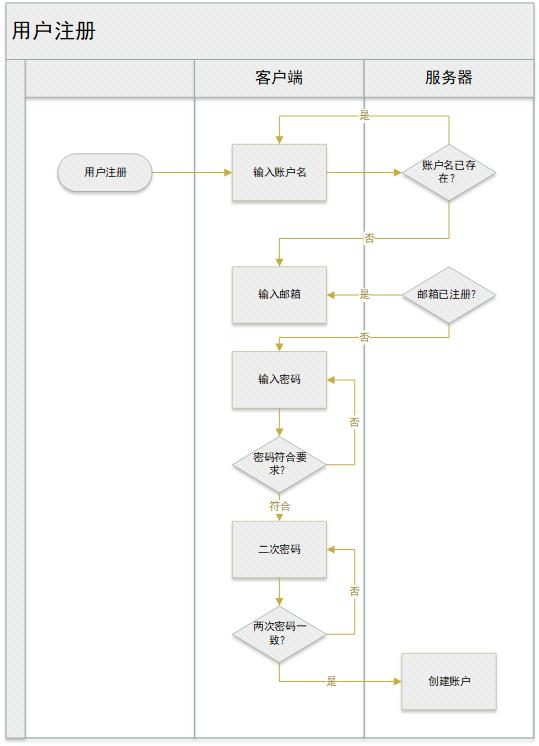
\includegraphics[scale=0.8]{Chapters/UML/user_register.jpg}
	\caption{用户注册流程图}
	\label{user_register}
\end{figure}

\cref{user_release}是用户发布图书流程图。用户在客户端选择扫描条形码或手动输入来获取图书 ISBN,然后
请求应用服务器获取图书相关信息,如果应用服务器没有该书信息,则应用服务器请求三方服务器获取图书信息,成功
获取到后,首先保存在本地应用服务器中,然后返回给客户端相关的图书信息。客户端获取到图书信息后,进一步补充
相关信息,然后再次发送请求到应用服务器,完成发布。

\begin{figure}[h]
	\centering
	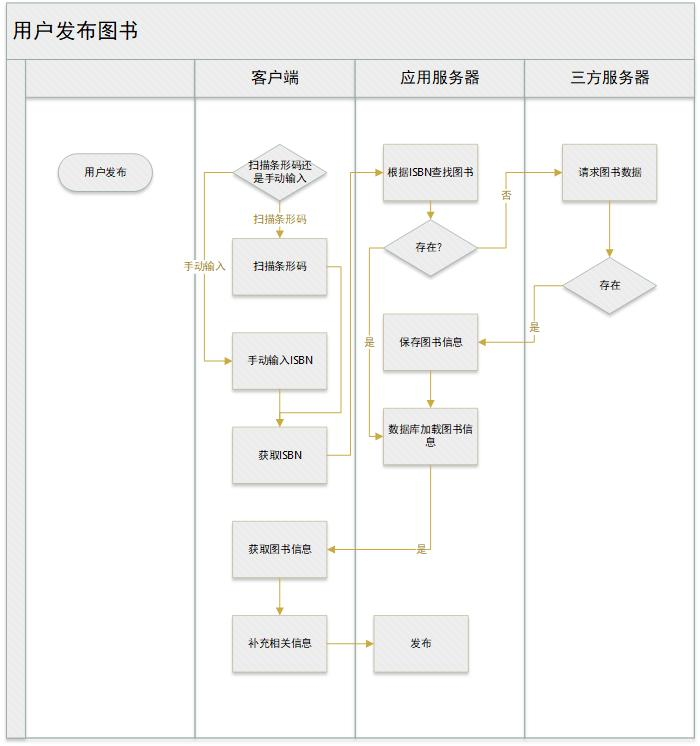
\includegraphics[scale=0.7]{Chapters/UML/user_release.jpg}
	\caption{用户发布流程图}
	\label{user_release}
\end{figure}

\cref{user_rent_or_buy}是用户租赁购买图书流程图。用户在客户端选择租赁或购买,请求应用服务器,服务器生成
响应的订单信息并返回。用户在客户端选择订单进行支付,服务器根据用户账户余额来判断是否能够完成支付。如果支付
完成,则订单进入约定交付状态,用户和图书拥有者通过沟通交付订单。如果是购买,则当用户点击收获后订单完成。否则,
如果是租赁,则订单进入待归还状态,在图书拥有着点击确认归还后,订单完成。

\begin{figure}[p]
	\centering
	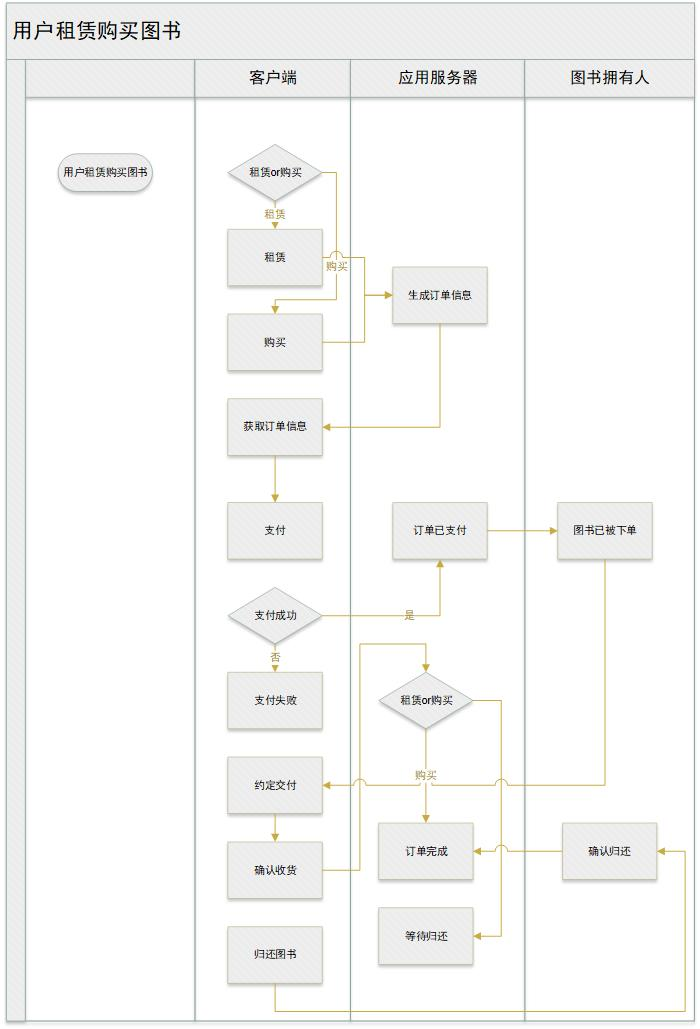
\includegraphics[scale=0.75]{Chapters/UML/user_rent_or_buy.jpg}
	\caption{用户租赁购买图书流程图}
	\label{user_rent_or_buy}
\end{figure}

\section{ Android 客户端界面与功能设计}
\cref{android_ui}是 Android 客户端功能设计。

未登录用户可以通过首页查看图书列表,和图书详情信息,但是不能发布图书。

登录用户拥有未登录用户的所有功能,并且可以发布图书,以购买或租赁图书的方式下单并进行支付。

根据设计和需求分析,将客户端划分为以上用户界面,下面对各个界面进行介绍:

\subsection{首页}

\begin{figure}[h]
	\centering
	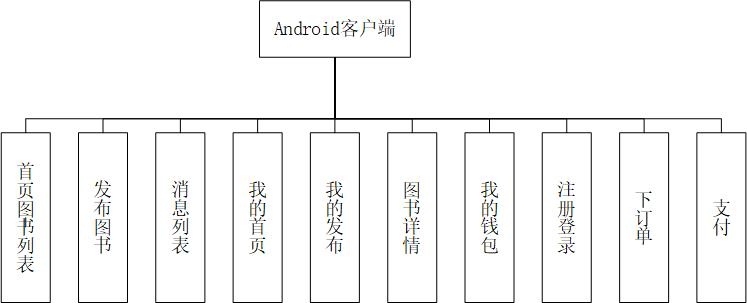
\includegraphics[scale=0.7]{Chapters/UML/android_ui.jpg}
	\caption{移动端界面功能设计}
	\label{android_ui}
\end{figure}

\cref{main_ui}是 Android 的客户端主页,包含图书列表和最下方的导航栏。用户通过下滑操作查看图书列表,通过点击某项,
	查看图书具体信息。
	
	\begin{figure}[h]
		\centering
		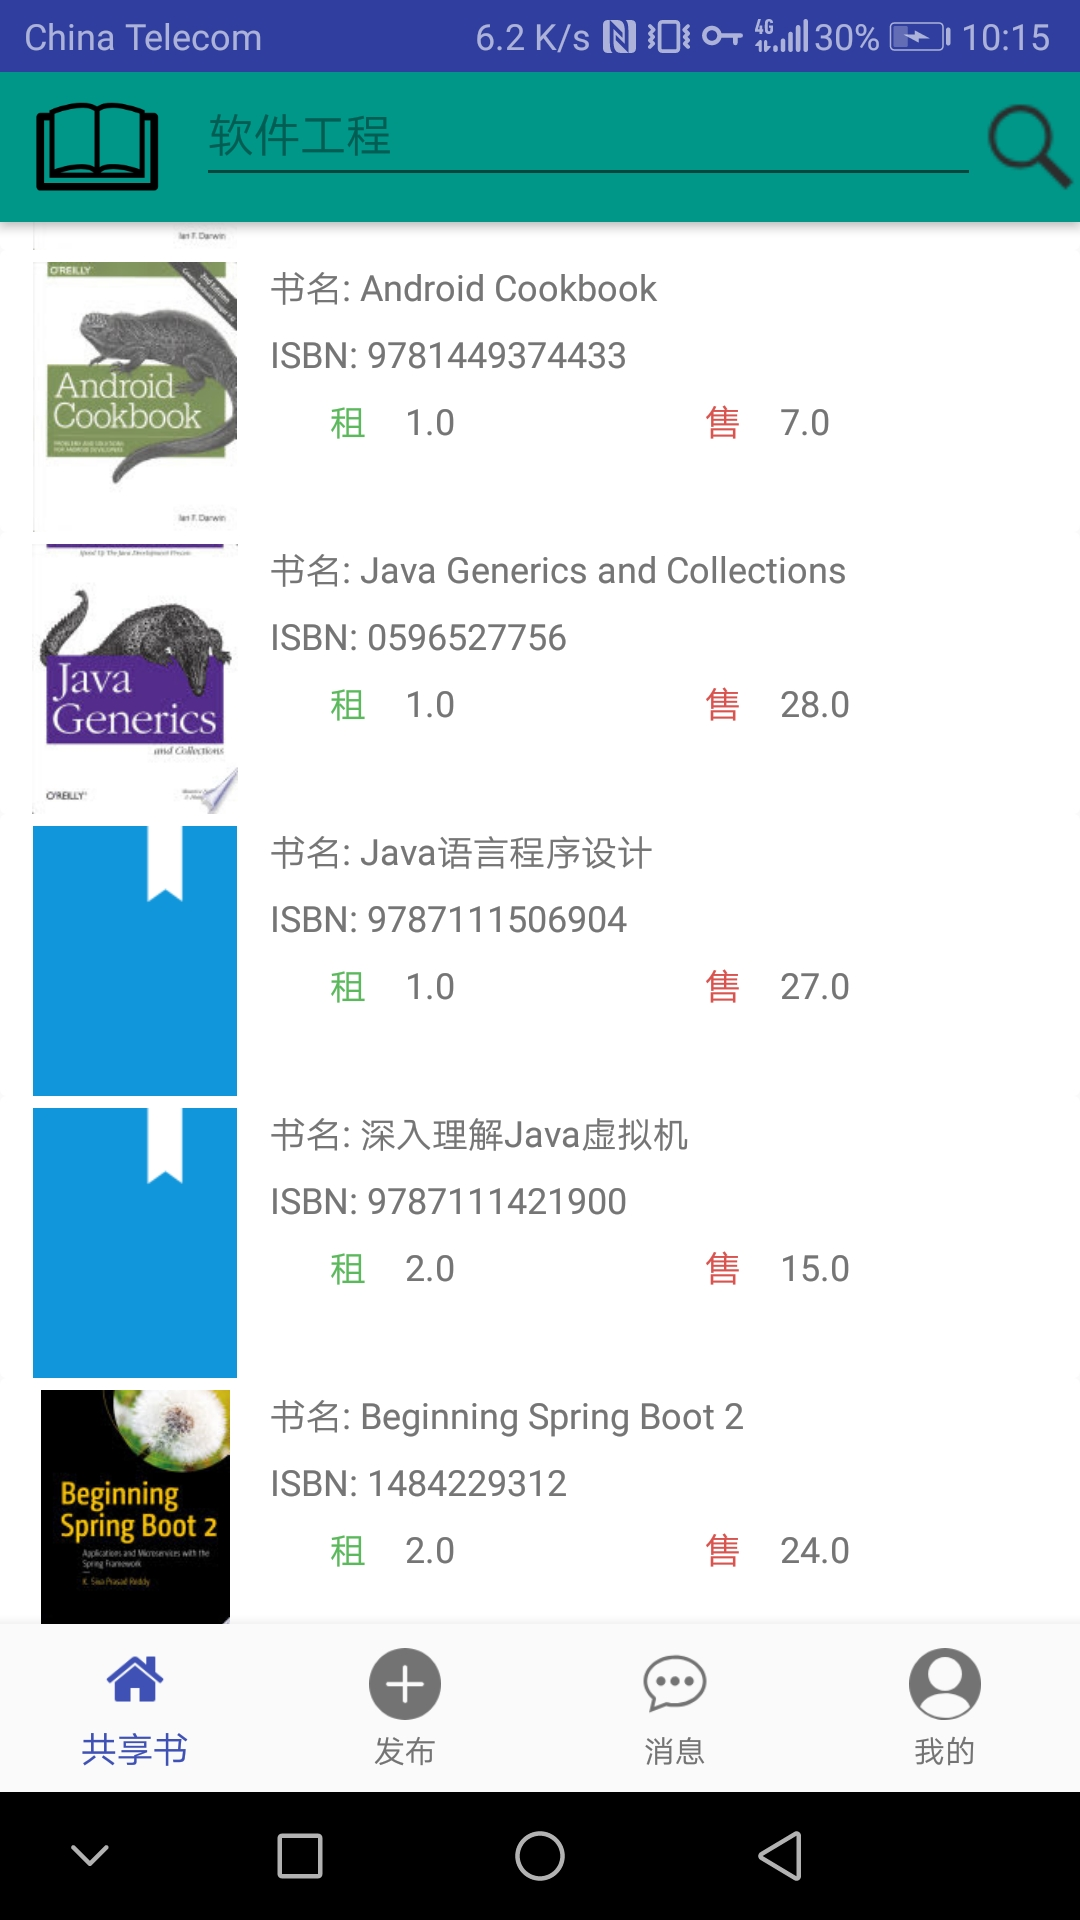
\includegraphics[scale=0.09]{Chapters/UI/book_list.jpg}
		\caption{客户端首页}
		\label{main_ui}
	\end{figure}

	导航栏是 App 的主要功能入口,导航栏有四个选项:共享书,发布,消息,我的。共享书对应 App 的主页,发布对应发布
	选项,消息对应最近联系人页面,我的对应与用户相关的页面。

\cref{self_intro}显示了个人主页,这里是与用户个人相关的页面,包括我的钱包,我的订单,我的发布,清除缓存 ,退出登录等。

\begin{figure}[h]
	\centering
	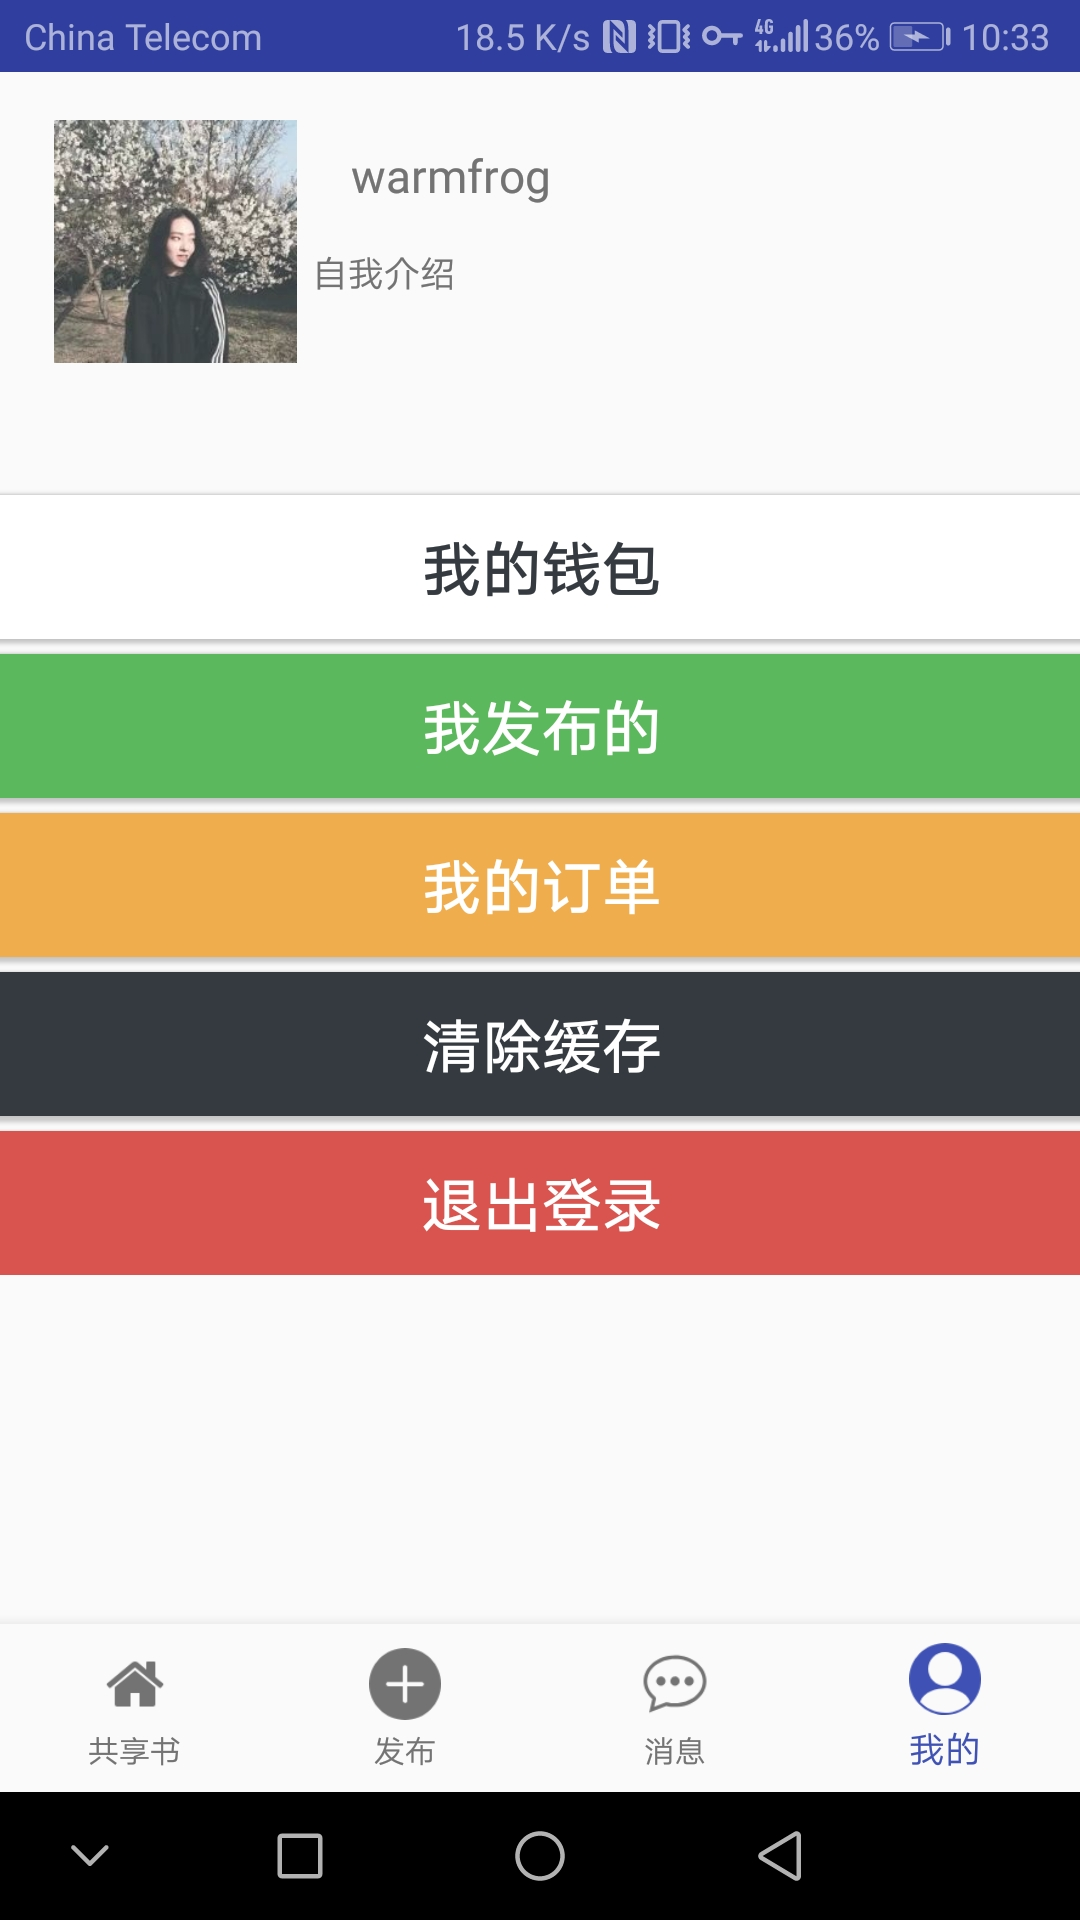
\includegraphics[scale=0.09]{Chapters/UI/self_intro.jpg}
	\caption{个人主页}
	\label{self_intro}
\end{figure}

\cref{unlogin}是用户未登录时进入点击我的导航栏时进入的页面,提示用户进行登录。

\begin{figure}[h]
	\centering
	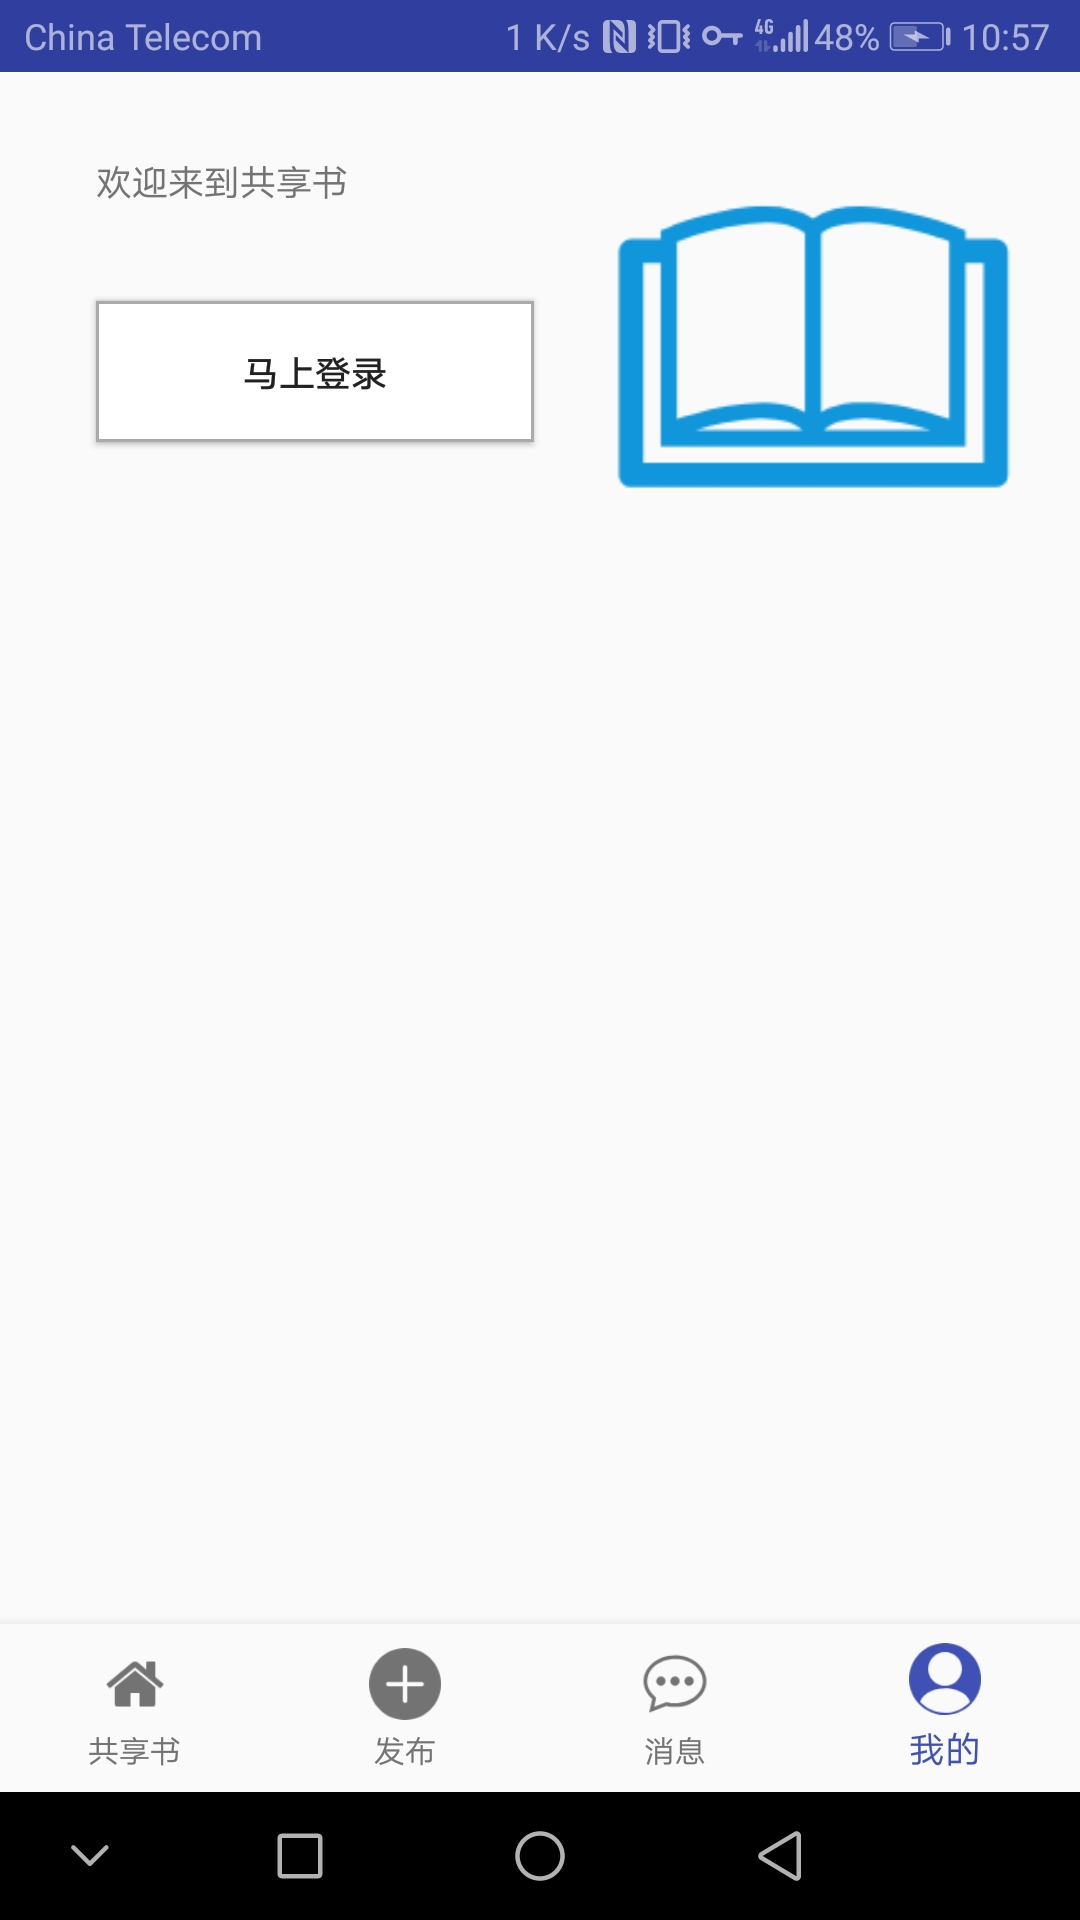
\includegraphics[scale=0.09]{Chapters/UI/unlogin.jpg}
	\caption{用户未登录}
	\label{unlogin}
\end{figure}

\subsection{用户模块}
\subsubsection{登录功能}
用户输入用户名或者注册邮箱和密码,点击是否记住账号和是否记住密码,当记住账号的复选框被勾选
时,用户账号会被记录到 Android 本地文件中;当记住密码的复选框被勾选时,用户密码也会保存到本地文件中。
用户点击登录,如果用户名不存在,将提示“用户名不存在,请注册”,如果密码不对,将提示账号或密码错误。
如果用户登录成功,则进入个人主页面。

\cref{login}是用户登录界面,用户通过输入注册时的用户名或者邮箱进行登录,如果密码不正确,或用户不存在,将提示用户重新登录或者注册。

\begin{figure}[h]
	\centering
	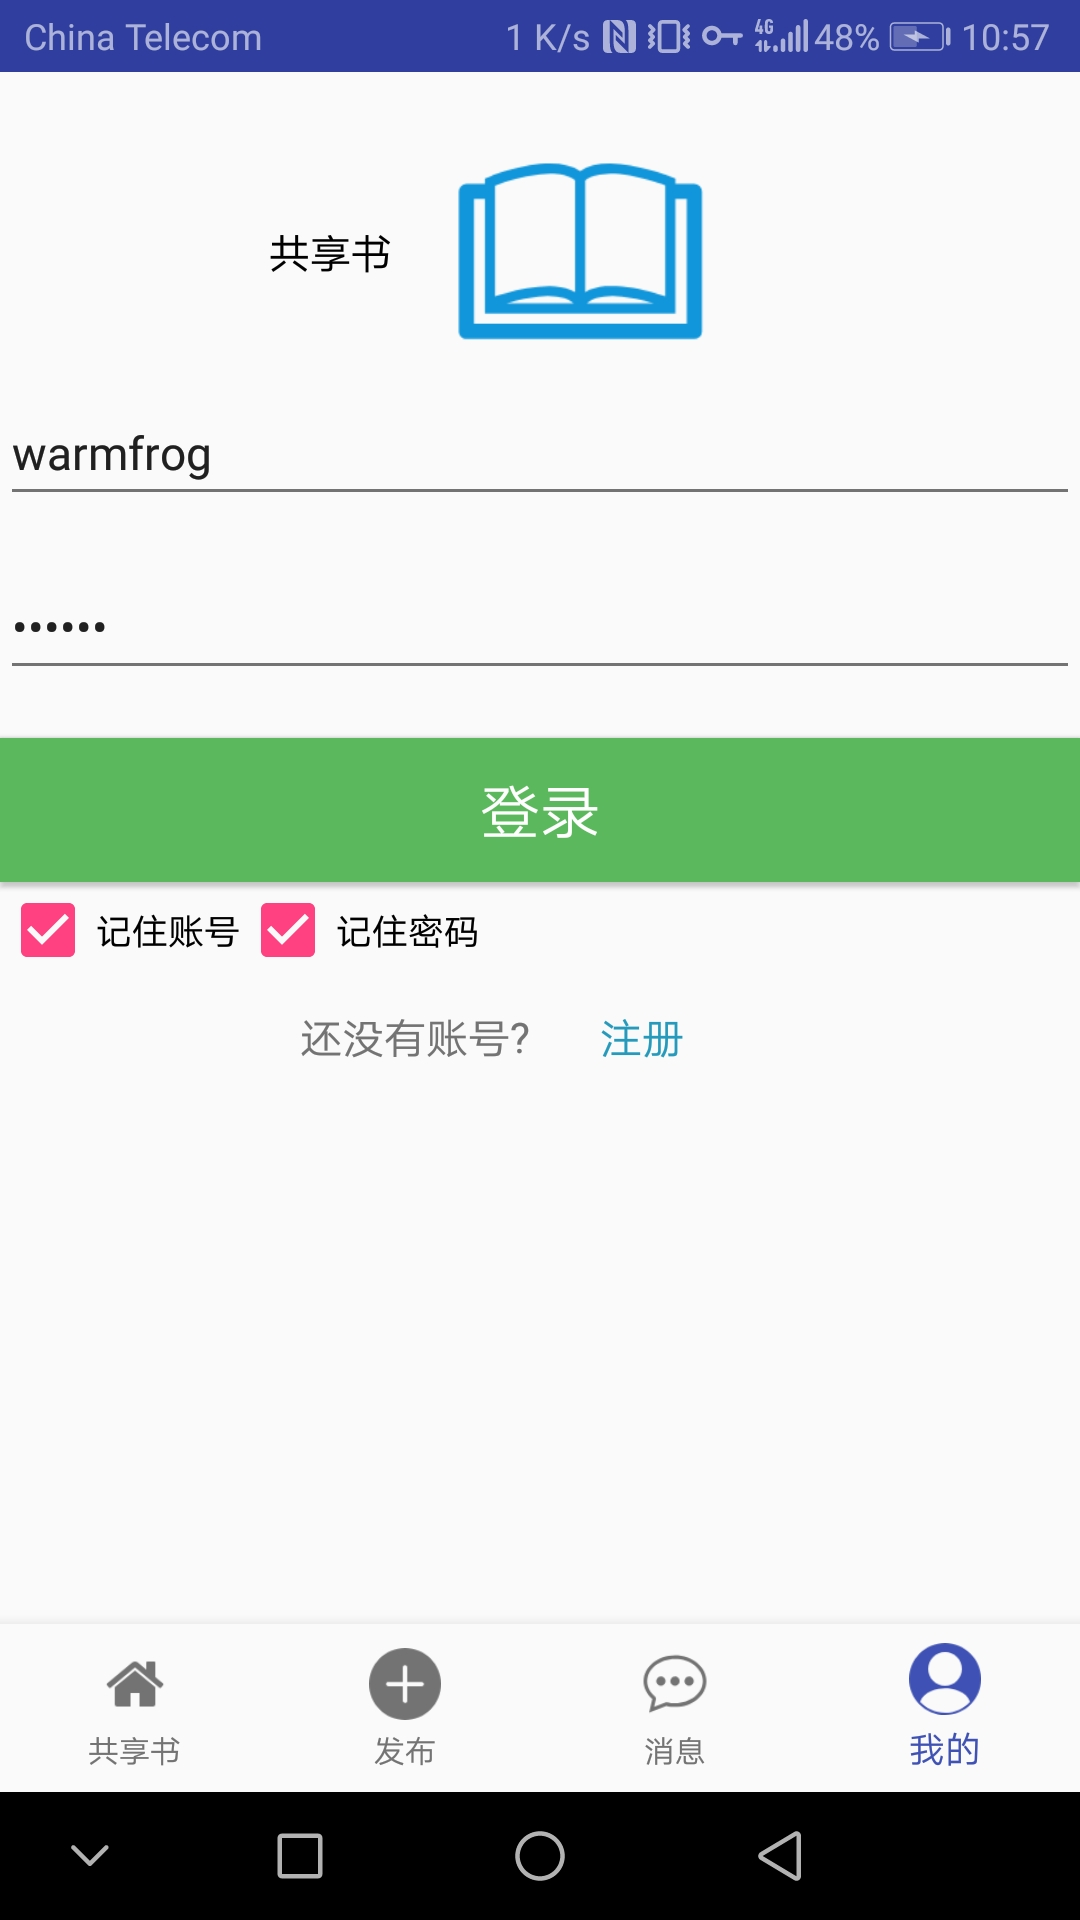
\includegraphics[scale=0.09]{Chapters/UI/login.jpg}
	\caption{登录}
	\label{login}
\end{figure}



\subsubsection{注册功能}
\cref{register}是用户注册页面,用户在该页面输入用户名,邮箱,密码等信息注册。
如果用户已存在,将提示用户,该账号已存在。

\begin{figure}[h]
	\centering
	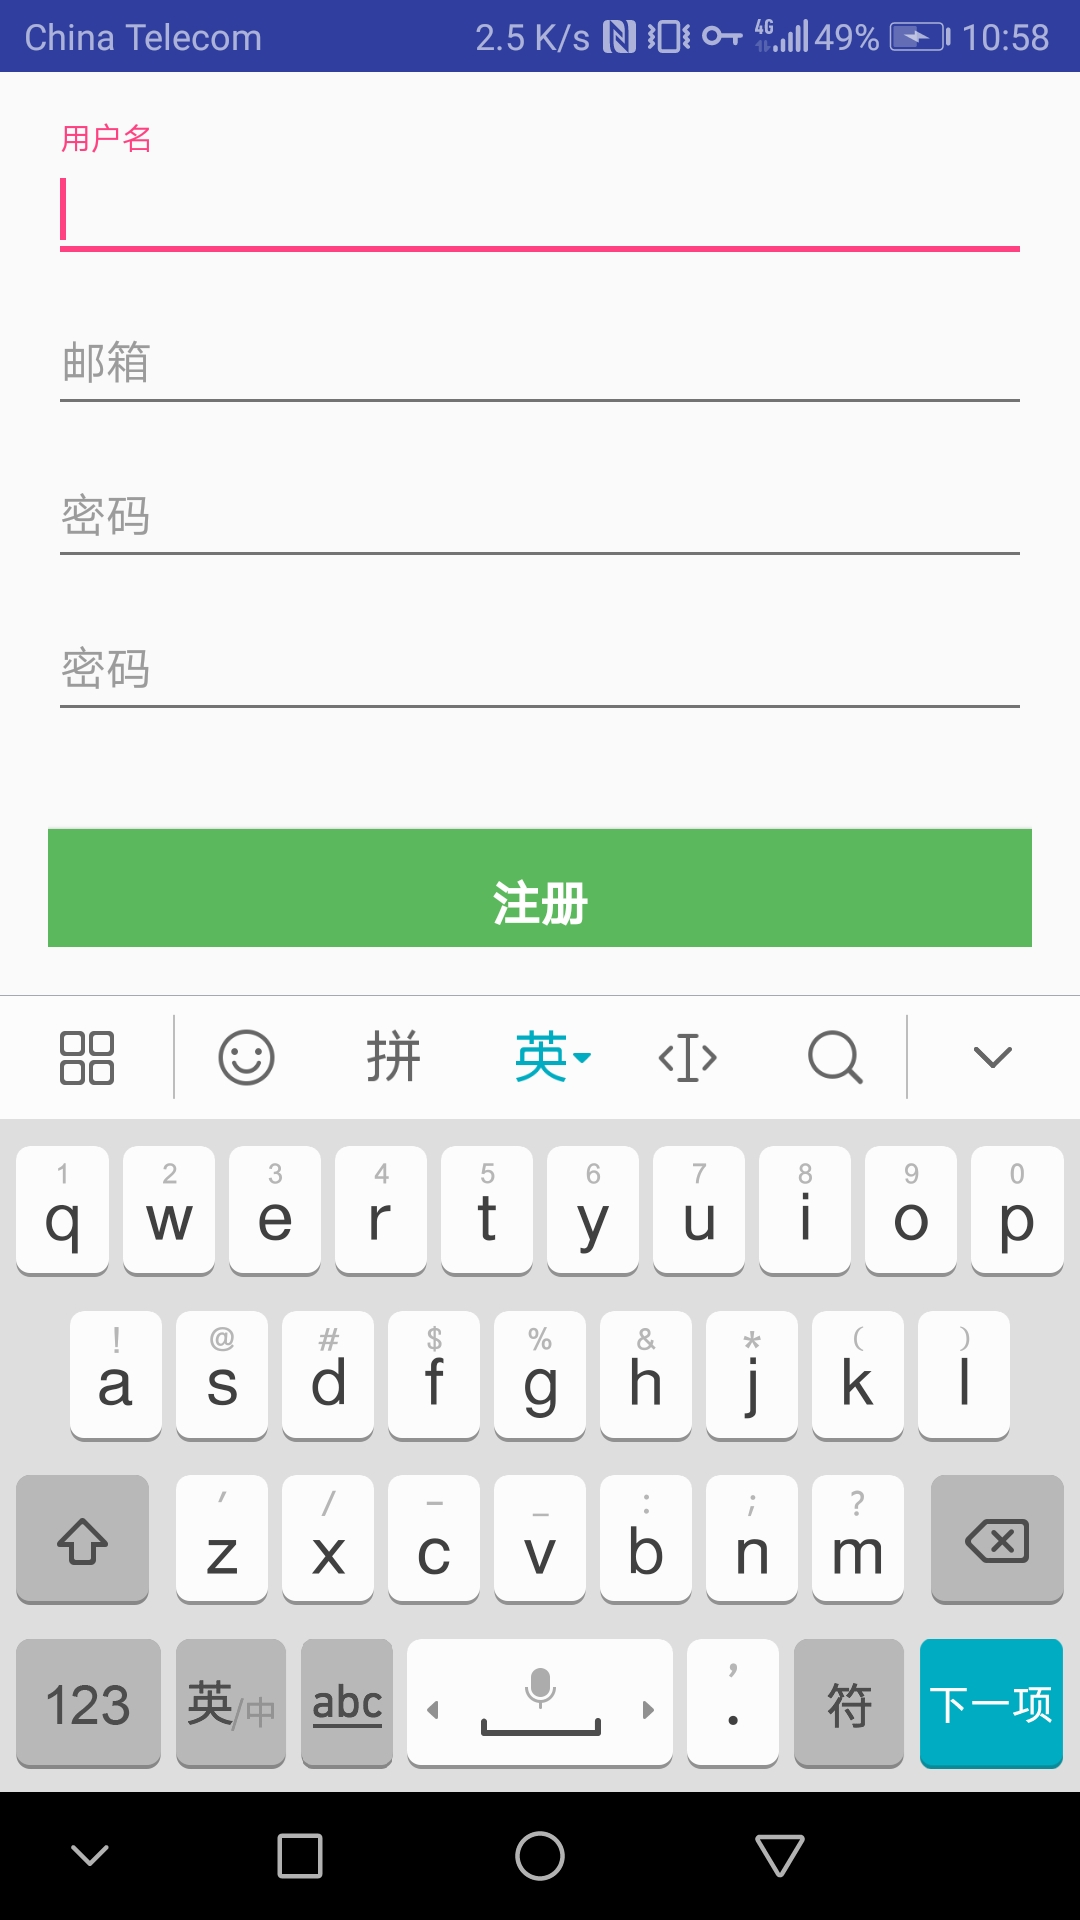
\includegraphics[scale=0.09]{Chapters/UI/register.jpg}
	\caption{注册}
	\label{register}
\end{figure}

用户进入登录界面,如果该用户没有账户,则可点击下方的提示注册按钮,进入注册页面。
用户在该页面输入用户名,邮箱,密码,确认密码信息。如果用户名或邮箱已经注册,将提示
该用户名或邮箱已经注册,请用户更换用户名或者登录。用户名和邮箱是绑定且唯一的。一个
邮箱只能注册一个账号。用户输入密码和确认密码,如果两次输入不一致,则提示用户两次输入
的密码不一致,请重新输入。




\subsection{发布图书}
用户点击发布图书,通过弹出的对话框,有两个选项。
一种方式是扫描条形码,用户点击该选项,将打开
一个 Activity 页面,该页面打开一个相机,中心是一个方形条形码区域,用户对准图书的条形码
区域,通过扫描,获取图书 ISBN;
另一个方式是手动输入图书的 ISBN。最终,用户将通过该 ISBN 获取该
书的所有相关信息,如果并未获取到该图书信息,下方弹出提示,未查询到该书信息,如果成功查询到该
书信息,将打开一个用户图书发布页面,该页面上方显示该书的详细信息,包括图书封面图片,图书 ISBN 信息,
图书的名称,图书的作者以及图书的出版时间信息,下方是用户自行补充的发布信息:包括租赁价格,出售价格
等。平台假定用户上传的图书都是可以租出和出售的。可选的,用户还可以输入相关描述信息,可以是图书推荐或者
图书使用情况。最终点击下方的发布按钮,完成图书发布。

用户点击发布时,有两种方式发布图书:一种是通过手机扫描图书条形码,获取图书 ISBN 获取
图书信息,一种是通过手动输入图书 ISBN。如\cref{release}所示。

\begin{figure}[h]
	\centering
	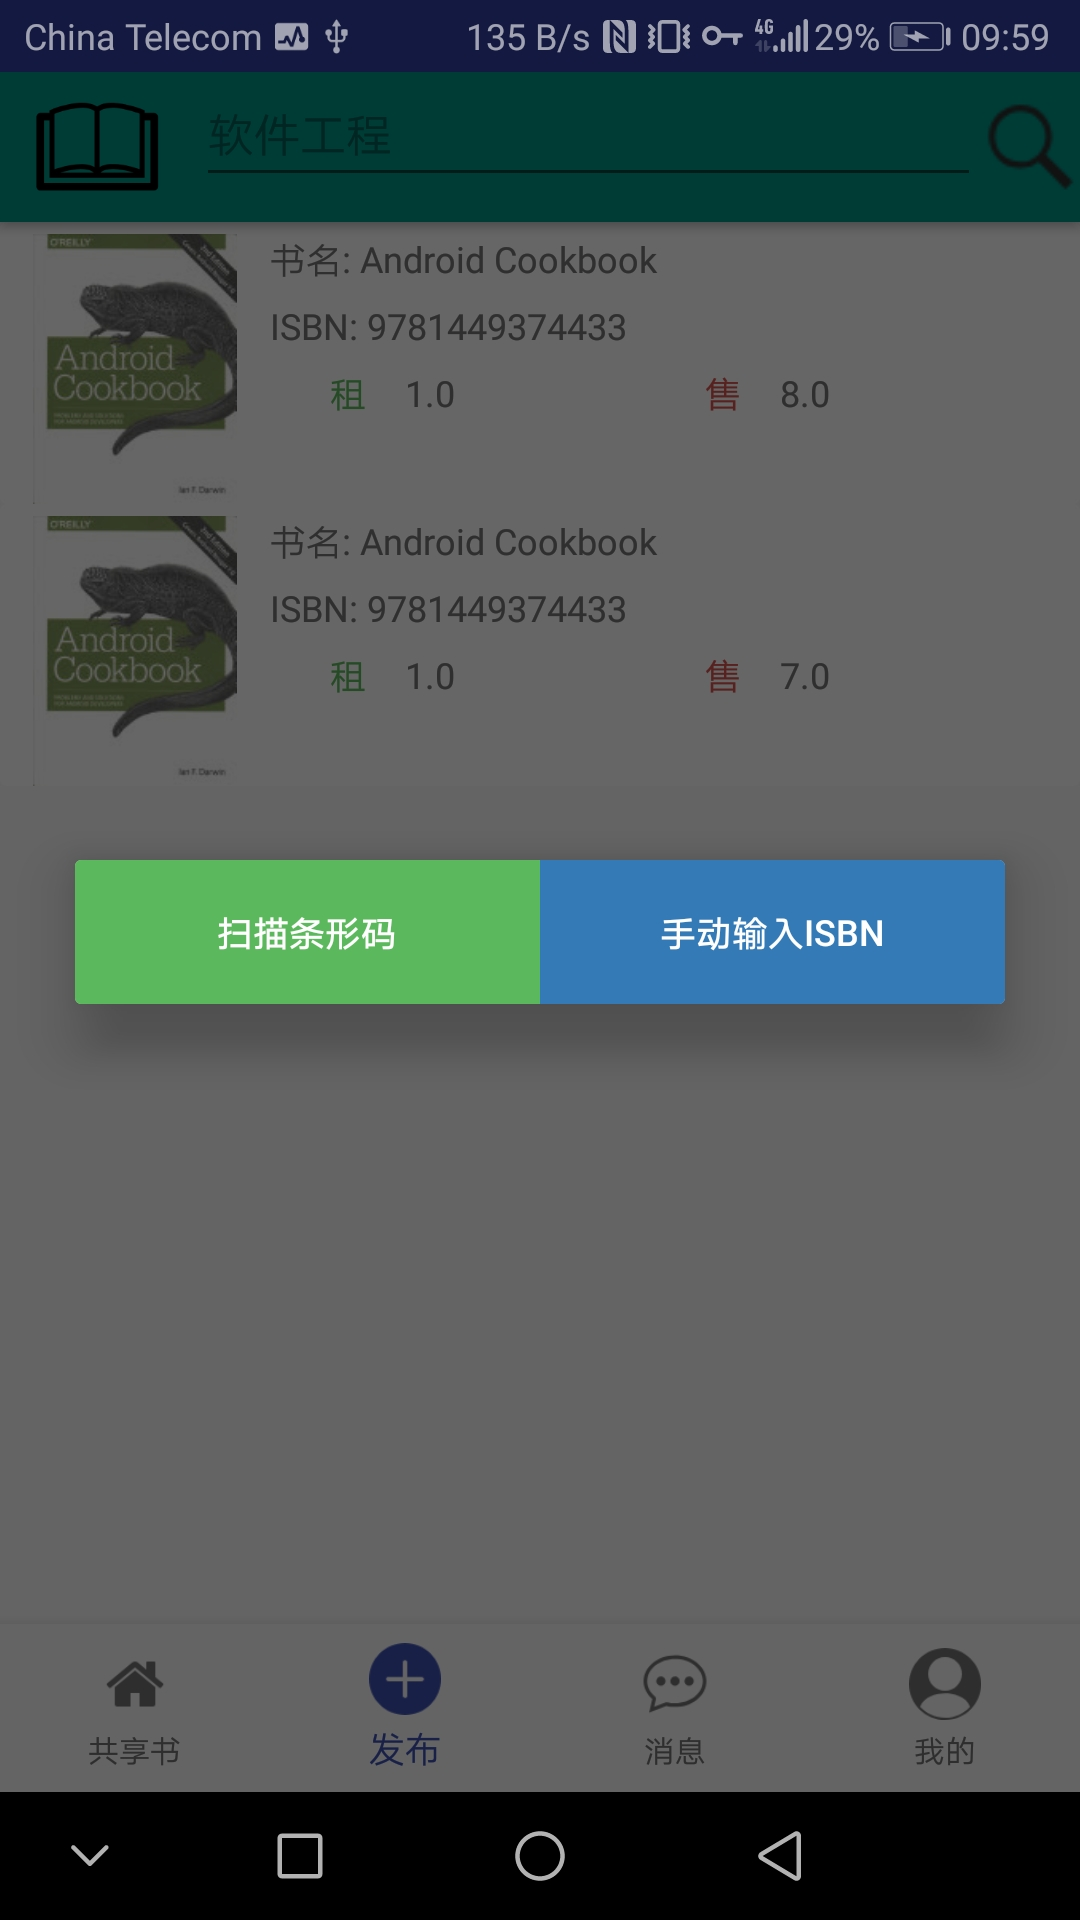
\includegraphics[scale=0.09]{Chapters/UI/release.jpg}
	\caption{点击发布}
	\label{release}
\end{figure}

\cref{scan}是用户点击发布后,选择扫描条形码时进入的页面,在该页面调用 Android
相机,扫描条形码,解析条形码,获取图书的 ISBN 信息,将 ISBN 发送到服务器,获取相应的图书信息。

\begin{figure}[h]
	\centering
	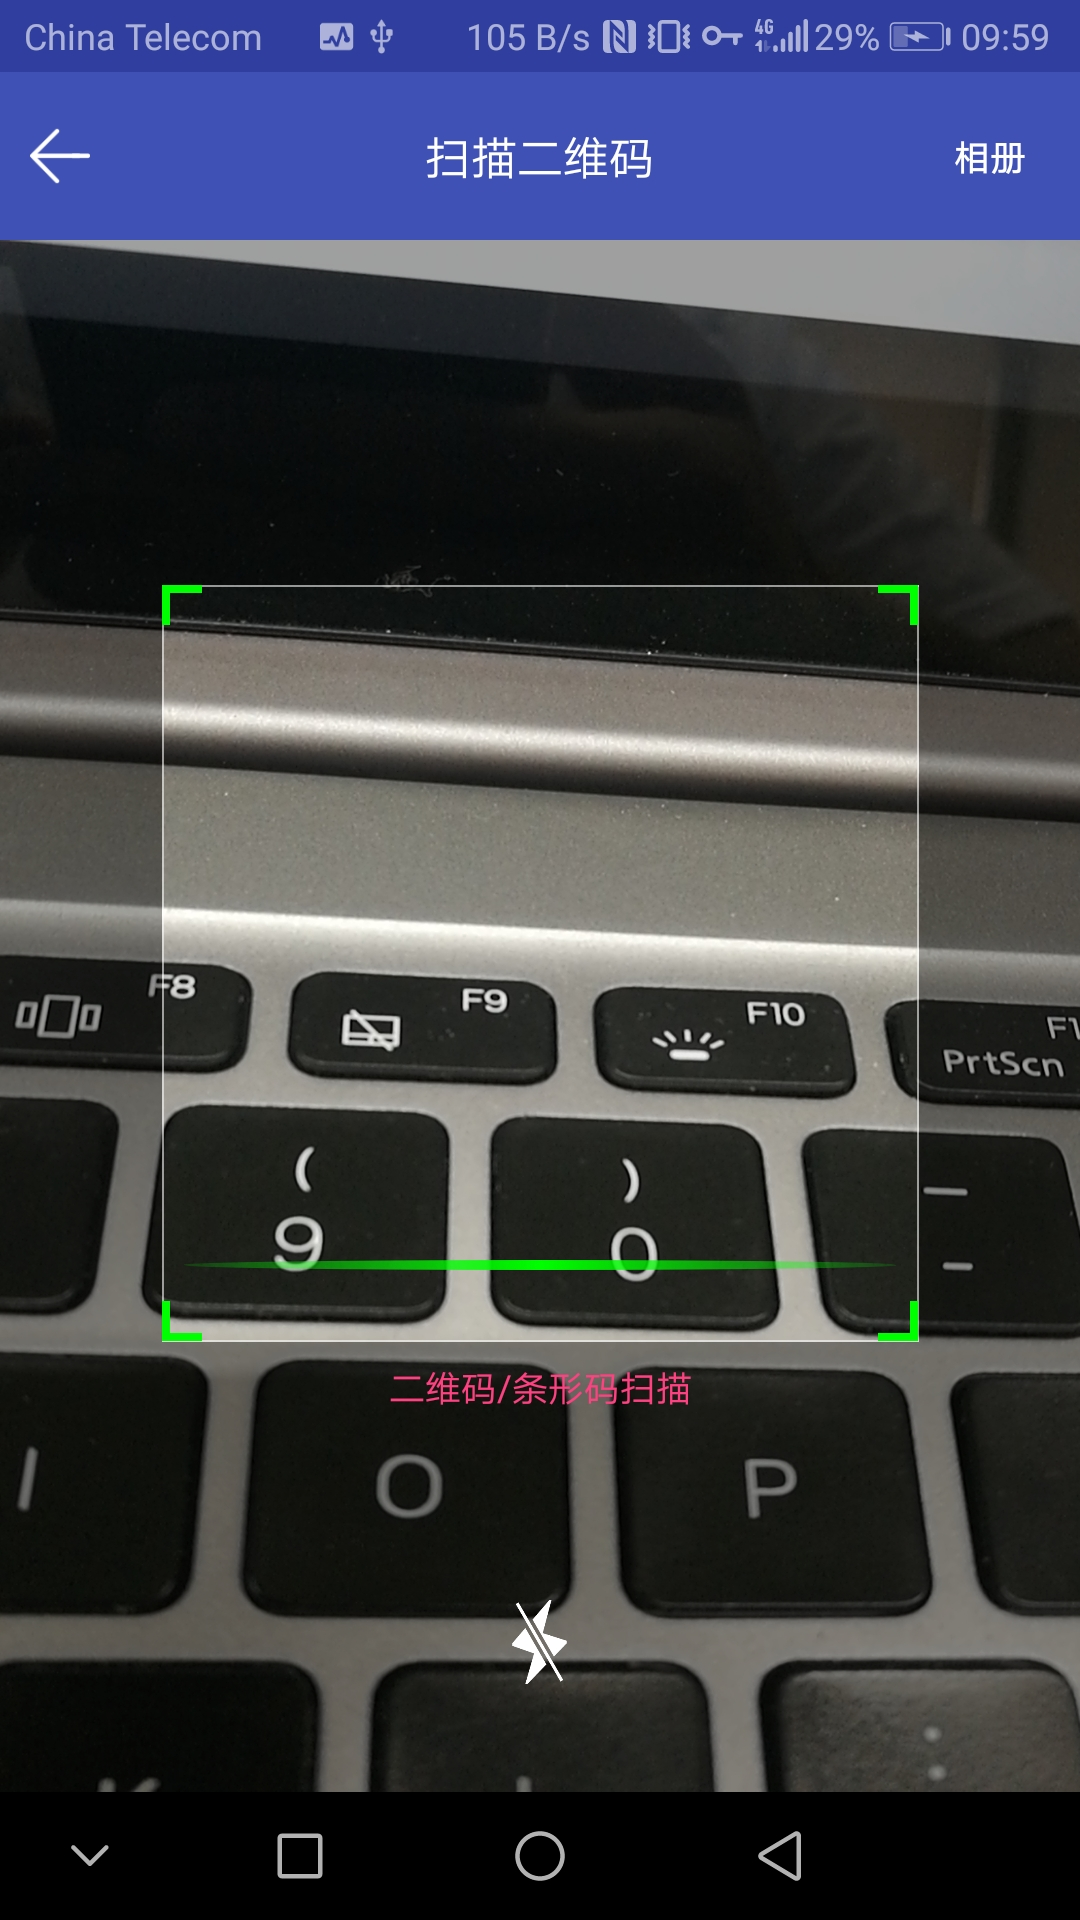
\includegraphics[scale=0.09]{Chapters/UI/scan.jpg}
	\caption{扫码图书条形码}
	\label{scan}
\end{figure}

\cref{input_isbn}是用户点击发布后,选择手动输入 ISBN 时进入的页面,用户在编辑栏手动输入图书的 ISBN 信息,发送到服务器来获得图书信息。

\begin{figure}[h]
	\centering
	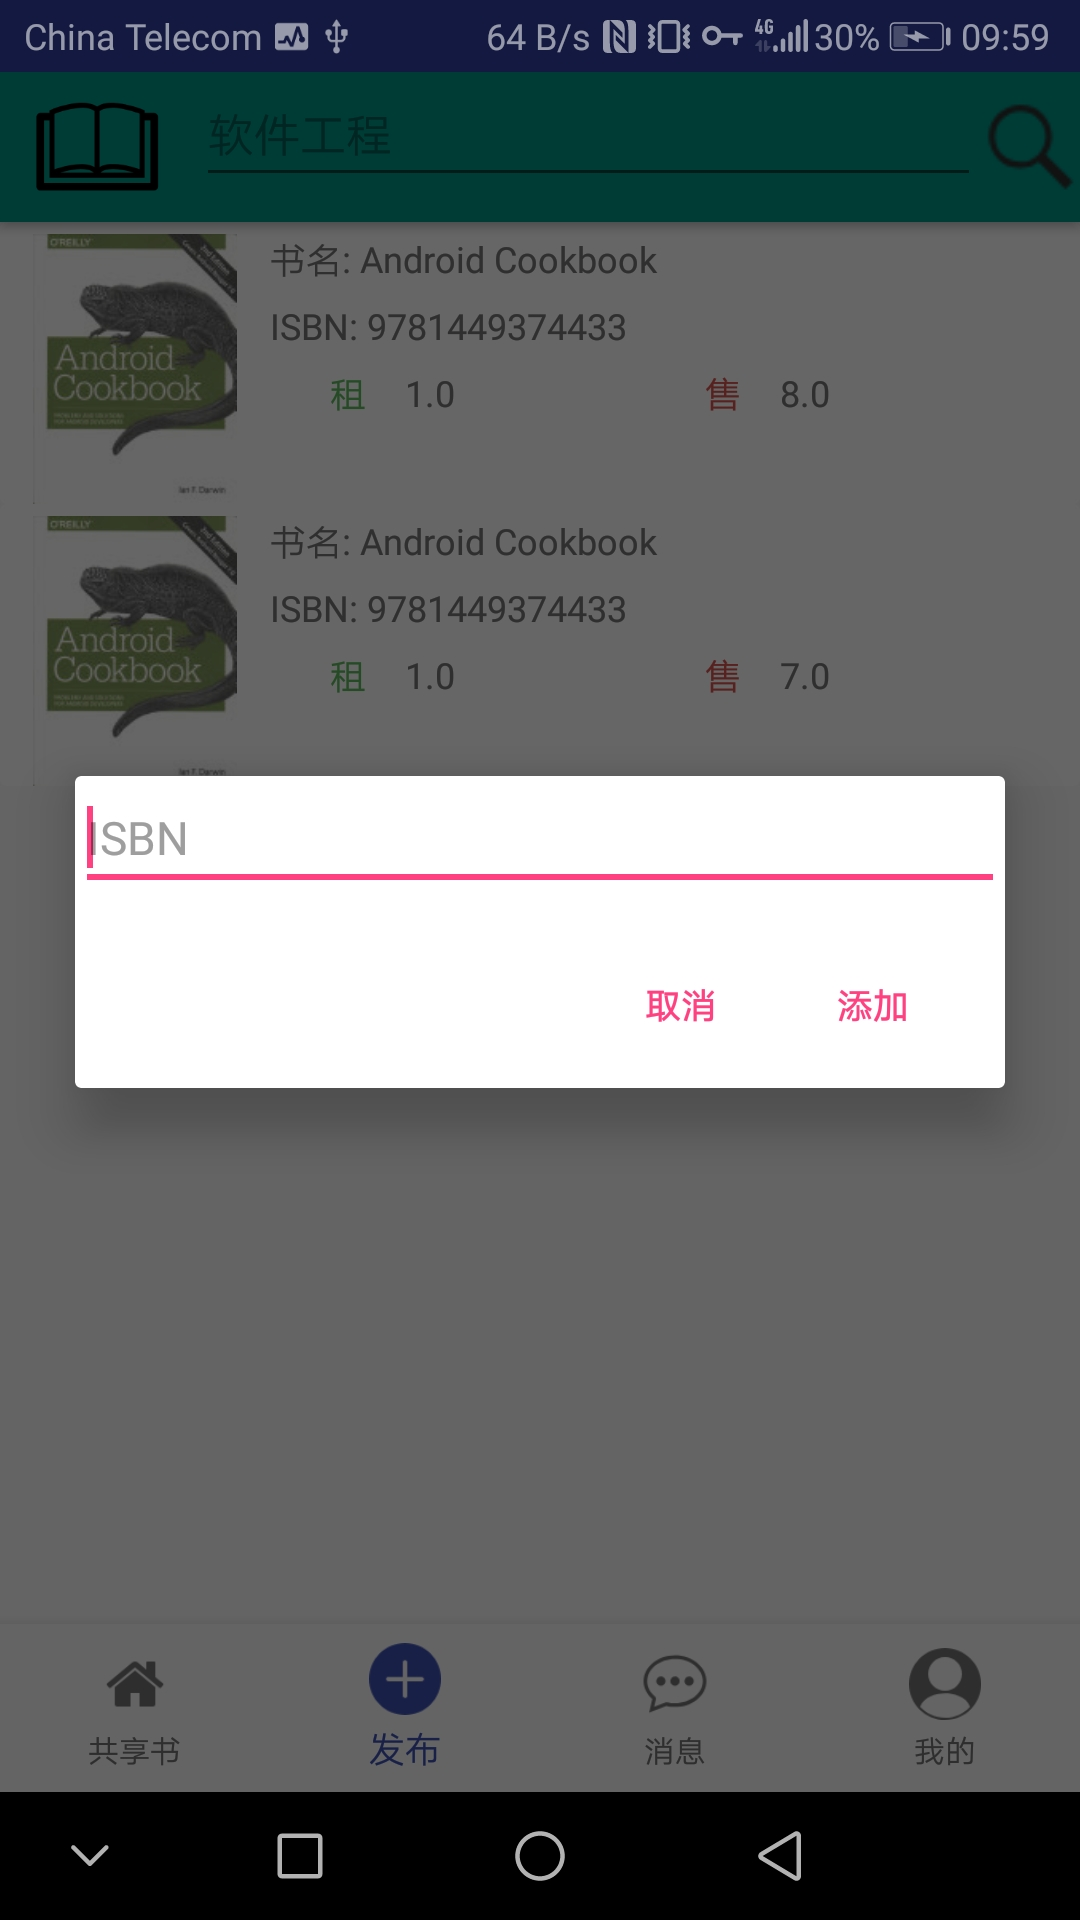
\includegraphics[scale=0.09]{Chapters/UI/input_isbn.jpg}
	\caption{手动输入图书ISBN}
	\label{input_isbn}
\end{figure}


\cref{release_from}是发布页面,用户点击发布,并从服务器获取到图书信息后,将进入此界面,用户进一步补充
相关的发布信息,如价格,个人平台或者描述等(可选),然后点击下方发布按钮进行发布。

\begin{figure}[h]
	\centering
	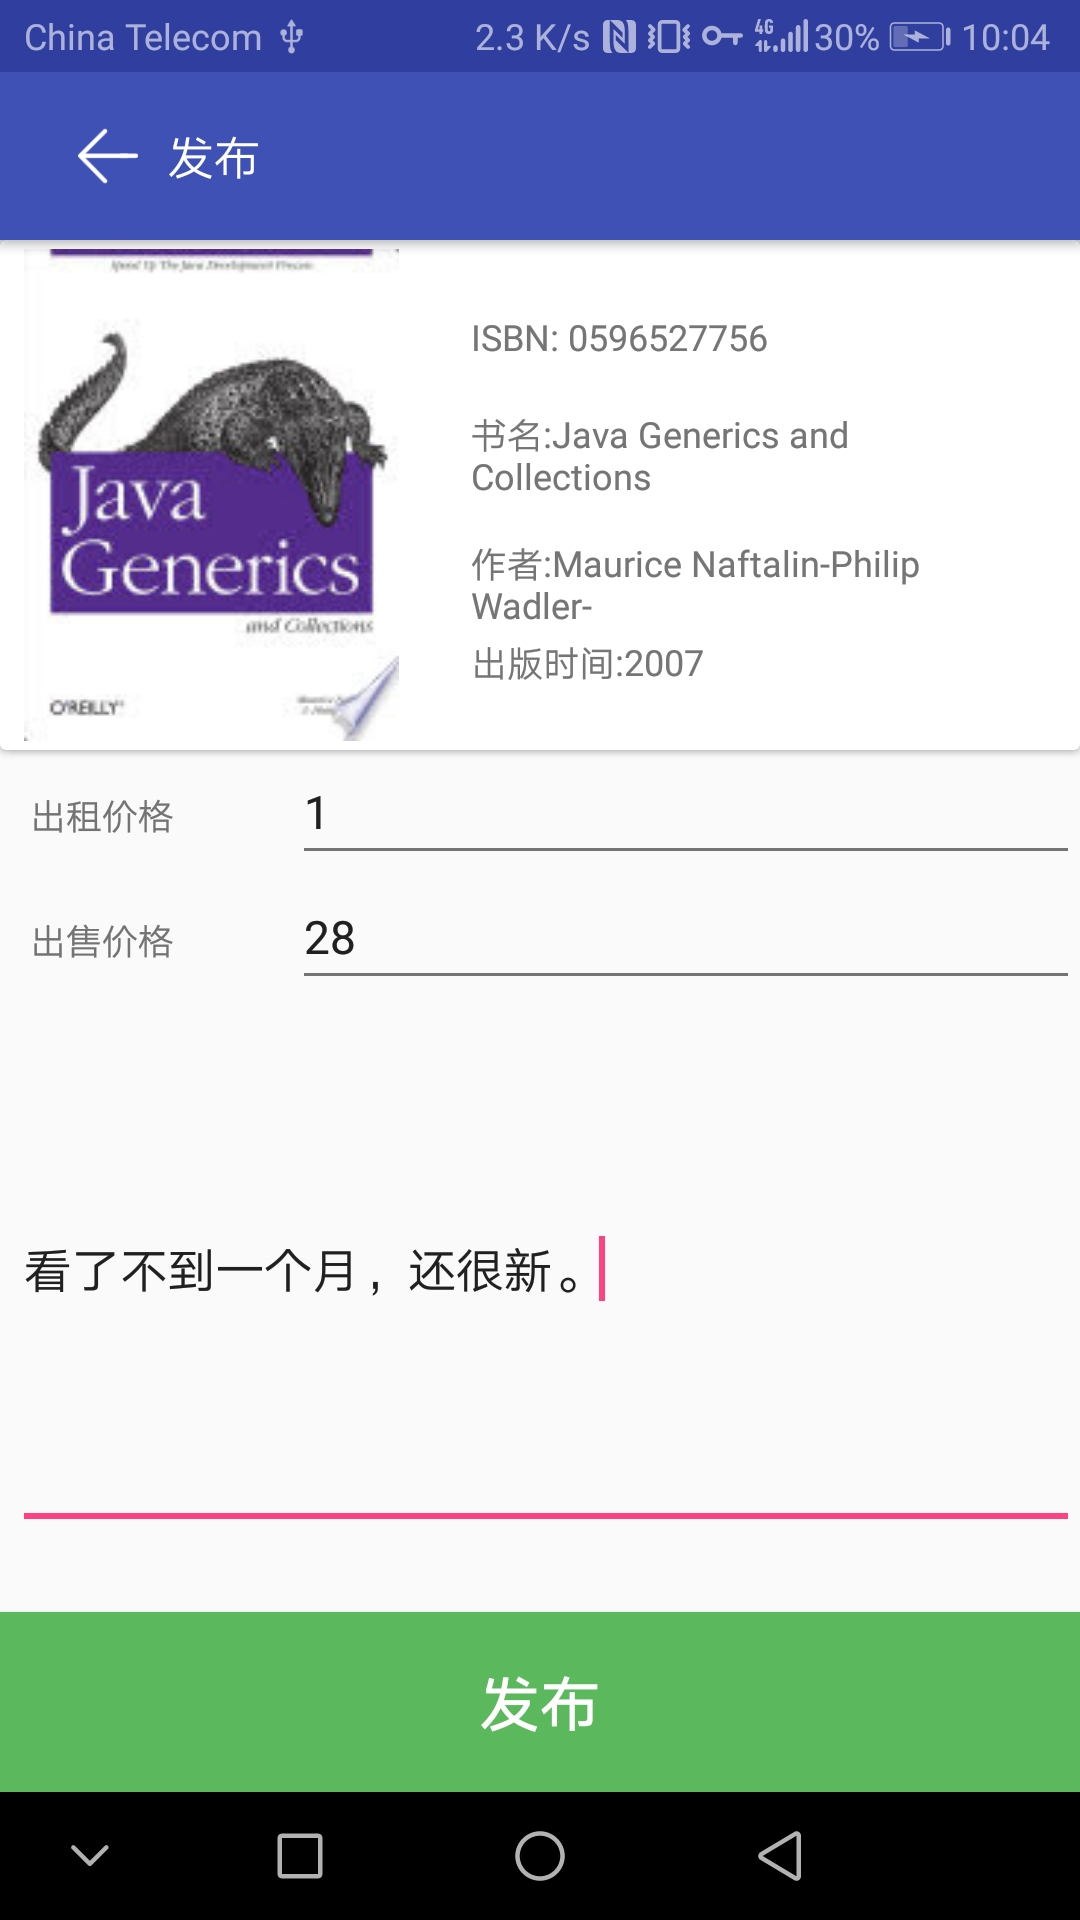
\includegraphics[scale=0.09]{Chapters/UI/release_form.jpg}
	\caption{补充发布信息}
	\label{release_from}
\end{figure}

\subsection{浏览图书}
用户打开主界面,主界面显示目前已加载的已发布的图书列表,列表的每一项包含少量的信息,包括图书封面,图书名,图书
ISBN,图书的租赁价格,图书的购买价格等信息。用户下拉,图书将持续加载,直至加载完所有图书。用户可以
通过点击某一项,查看自己感兴趣的图书的详细信息,并进行下一步操作。

\subsection{查看图书}

用户对某本书感兴趣,点击图书项后,打开一个新的 Activity 页面,该页面将显示该书的详细信息,上面是图书的基本信息,
包括图书封面,图书 ISBN,图书作者,图书名,出版时间,租赁价格,出售价格。中部是用户发布时的自行描述信息,下面
是图书的简介,最底部是两个选项,租赁、购买和聊一聊。用户点击租赁或购买时,会进入一个新的创建订单 Activity 页面,如\cref{order}所示。

\begin{figure}[h]
	\centering
	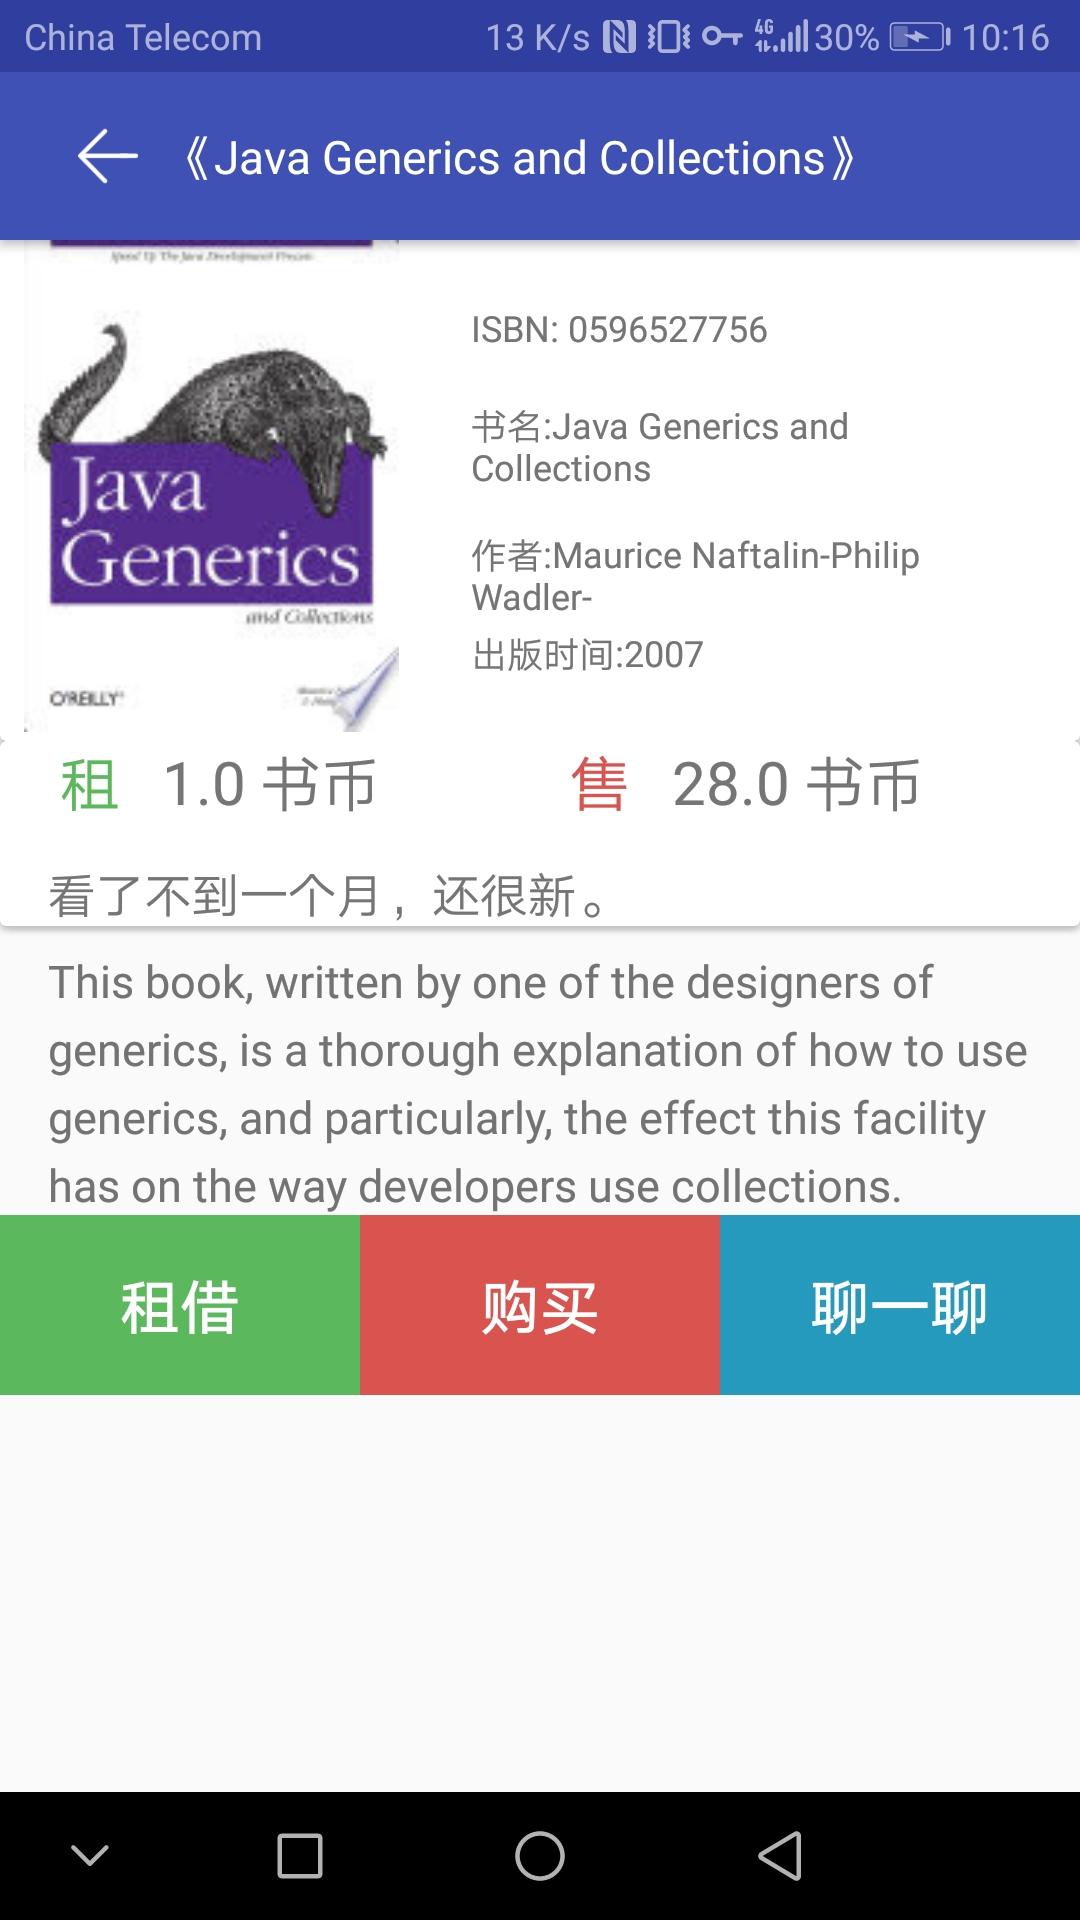
\includegraphics[scale=0.09]{Chapters/UI/ubook_info.jpg}
	\caption{图书详情}
	\label{ubook_info}
\end{figure}

当用户点击聊一聊时,打开一个聊天 Activity 界面,用户可以与图书主人聊天沟通,如\cref{talk}所示。

\cref{ubook_info}是图书详情信息,当用户点击图书某项时,会进入该页面,并显示图书详情信息,包括书名,ISBN,作者,描述等信息。

\begin{figure}[h]
	\centering
	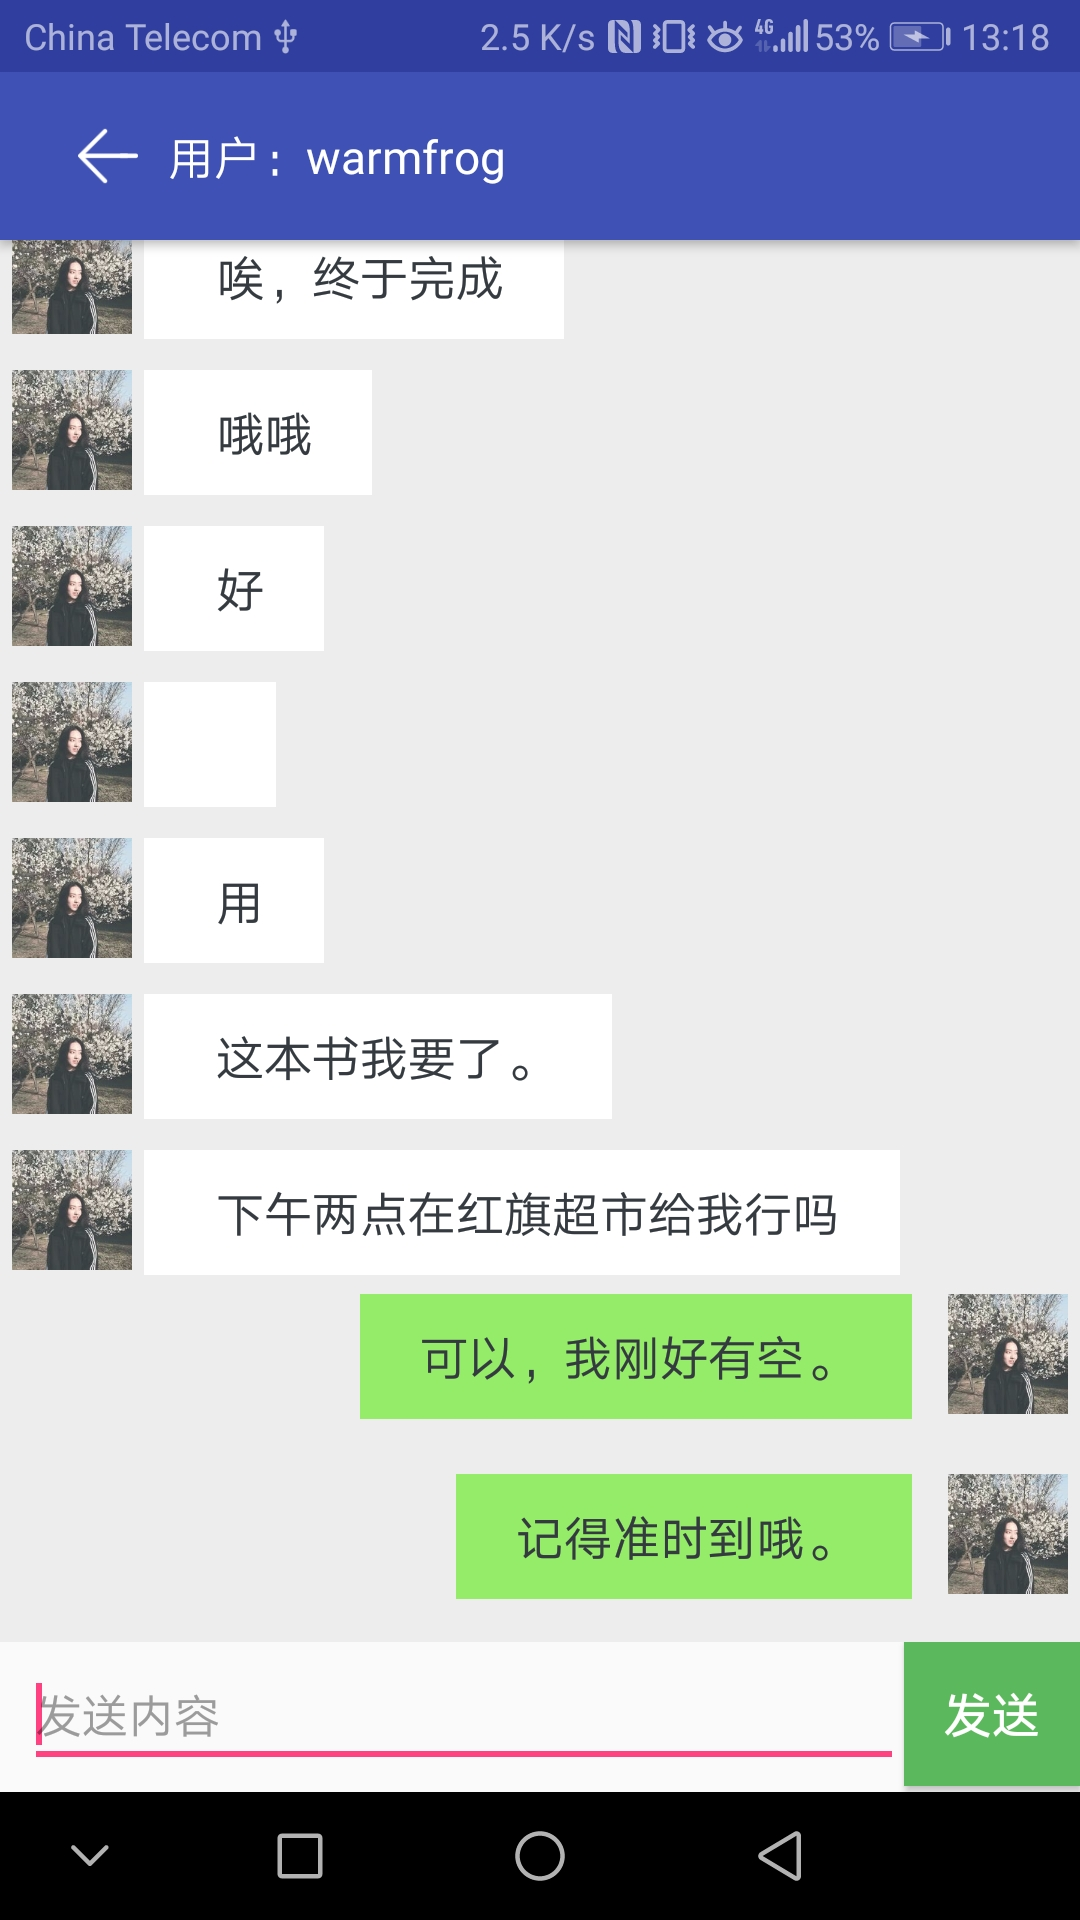
\includegraphics[scale=0.09]{Chapters/UI/talk.jpg}
	\caption{聊天沟通界面}
	\label{talk}
\end{figure}

\subsection{租赁购买图书}
\cref{order}是下单页面, 用户对某本书进行借阅或者购买时,会打开创建订单页面,上面是要下单的图书信息,封面,ISBN,作者,发布时间,下面是
从服务器获取的生成订单的信息,包括订单号,订单金额,订单时间,订单状态,订单类型等信息,最下面是要支付的总额
和立即支付按钮。用户点击支付,如果用户账户余额大于或者订单金额,将从用户账户扣除订单金额,并打开新的页面,提示用
户支付成功。否则,在新的页面提示用户支付失败。
相关的信息,会获取到服务器生成的订单号,

\begin{figure}[h]
	\centering
	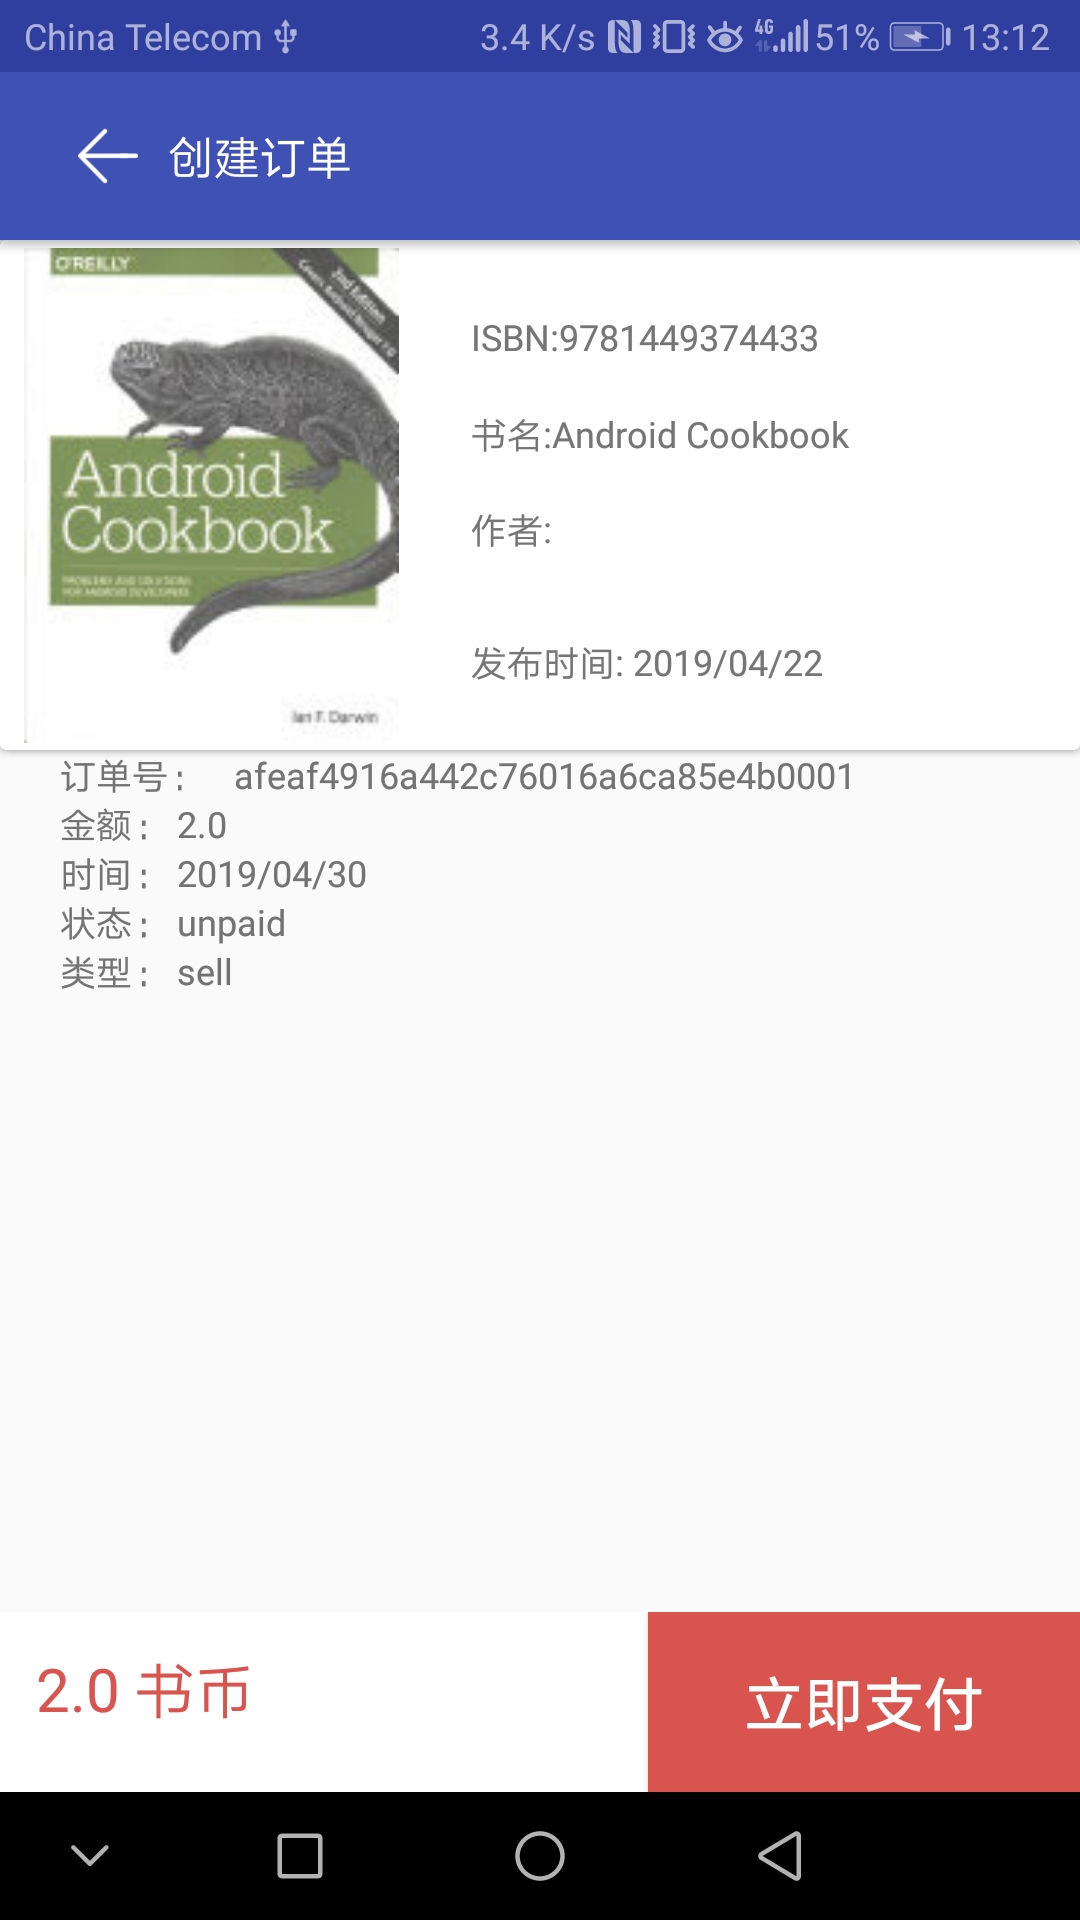
\includegraphics[scale=0.09]{Chapters/UI/order.jpg}
	\caption{下订单}
	\label{order}
\end{figure}

\subsection{管理图书}
用户在下方的导航栏点击我的-我发布的,进入我的发布页面。这也是一个图书列表,仅仅包含了当前登录用户的发布图书,每
一项包含图书封面,图书名,图书租赁价格,购买价格,发布时间和一个复选框。当用户点击某一项进入图书详情页,图书详情
页面包含详细的图书信息,包括图书封面,图书 ISBN,图书名,图书作者,出版时间,租赁价格,购买价格,用户自定义描述信息,
图书简介内容。页面最上面的动作栏包含一个返回按钮,图书的标题和帮助按钮。用户点击返回,将返回到图书列表页面。用户点击
帮助按钮,将在下方弹出帮助信息,提示用户选择要删除的项,并删除。帮助信息在两秒后自动消失。用户点击某一项的复选框时,
下方将弹出一个提示信息,提示用户是否删除该图书,如果用户点击删除,则将删除该书。如果用户无操作,提示信息在两秒后自行消失。

\cref{myubook}是我的发布页面。当用户在个人主页点击我的发布时进入该页面,显示该用户已发布的书籍列表。

\begin{figure}[h]
	\centering
	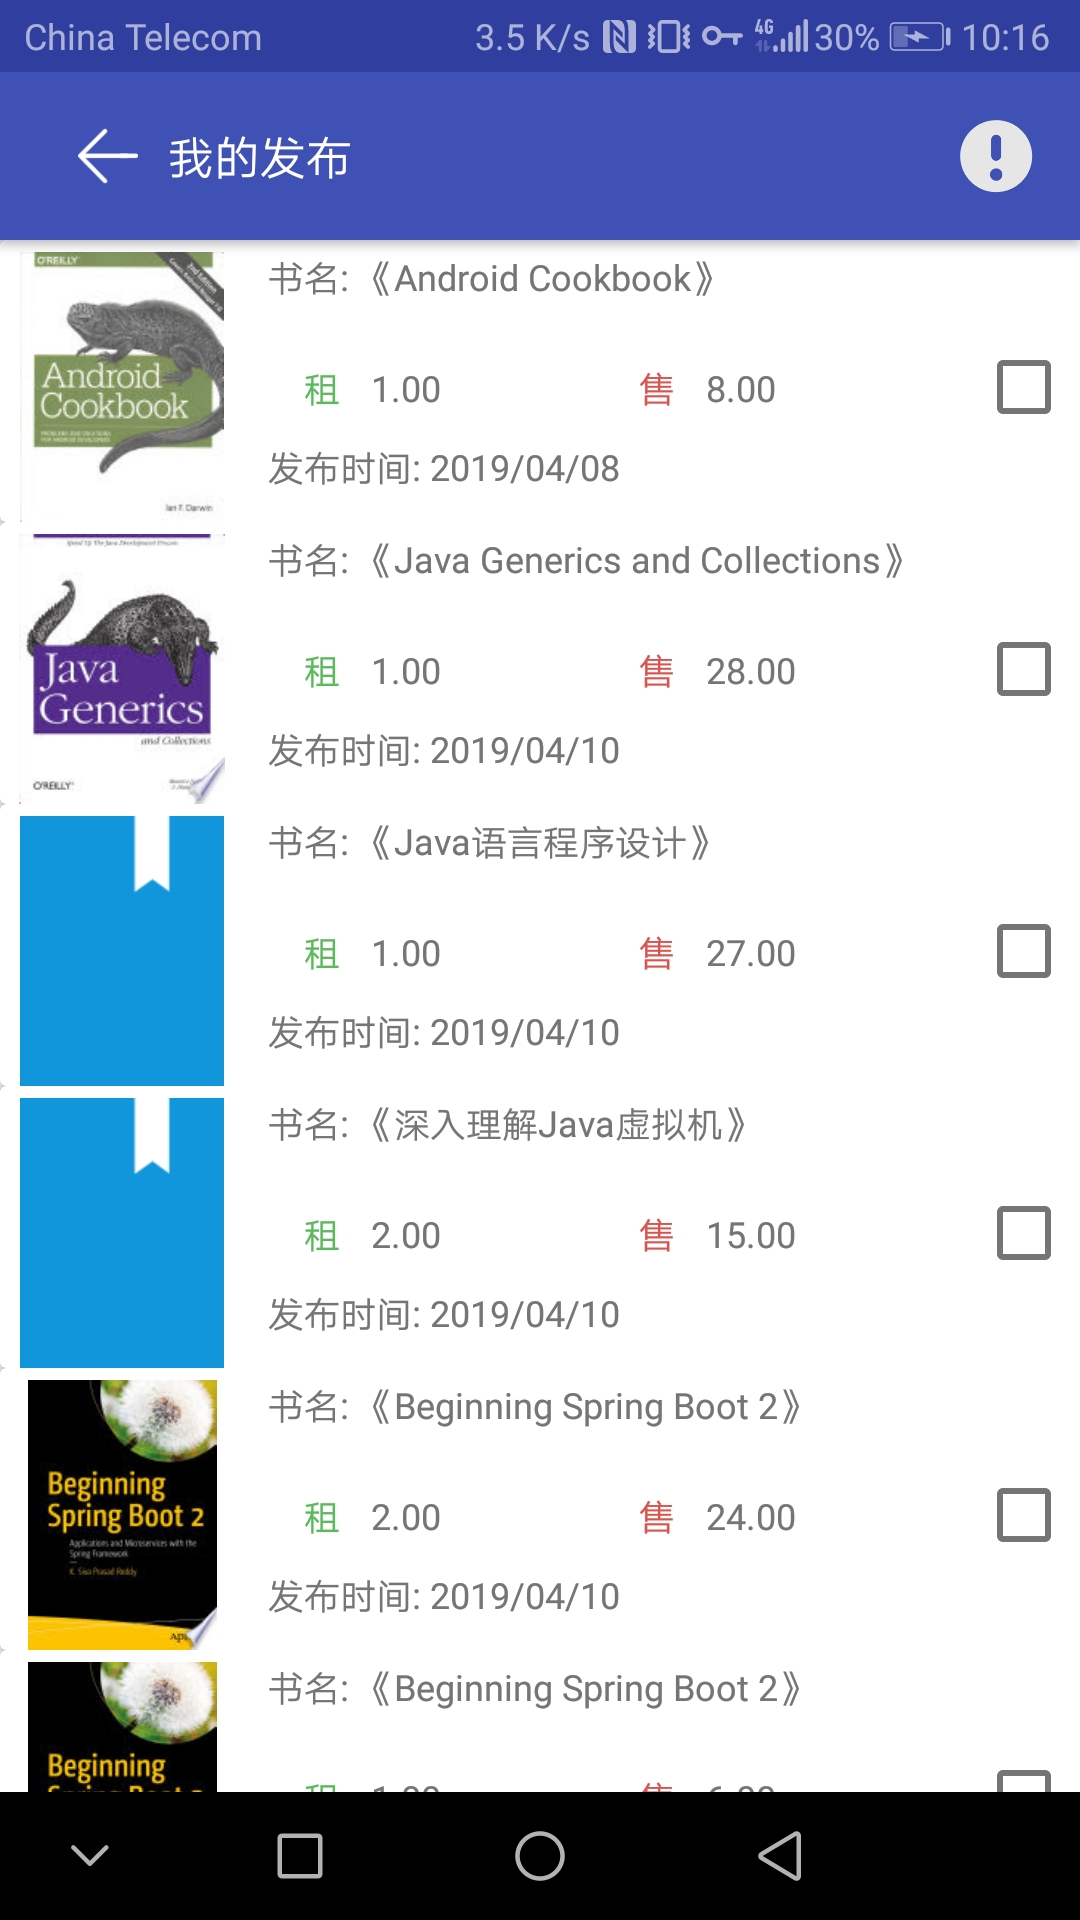
\includegraphics[scale=0.09]{Chapters/UI/myubook.jpg}
	\caption{我的发布}
	\label{myubook}
\end{figure}

\subsection{订单管理}
用户在下方的导航栏,我的-我的订单,进入我的订单页面。这里将显示用户所有的订单信息。订单页面动作栏显示一个返回按钮和标题
我的订单。用户点击返回按钮,将返回我的个人主页。订单页面包含订单列表。每一项包含订单的详细信息,分为三个区域上中下。上区域
最上面显示该订单中图书的拥有者信息,订单的状态。上区域的下面包含该订单中的图书信息,包含图书封面,图书标题,图书 ISBN。中
区域包含订单信息,包含订单号,订单金额,下单时间,订单状态,订单类型。下区域是两个按钮,包含对订单的操作。

\begin{figure}[h]
	\centering
	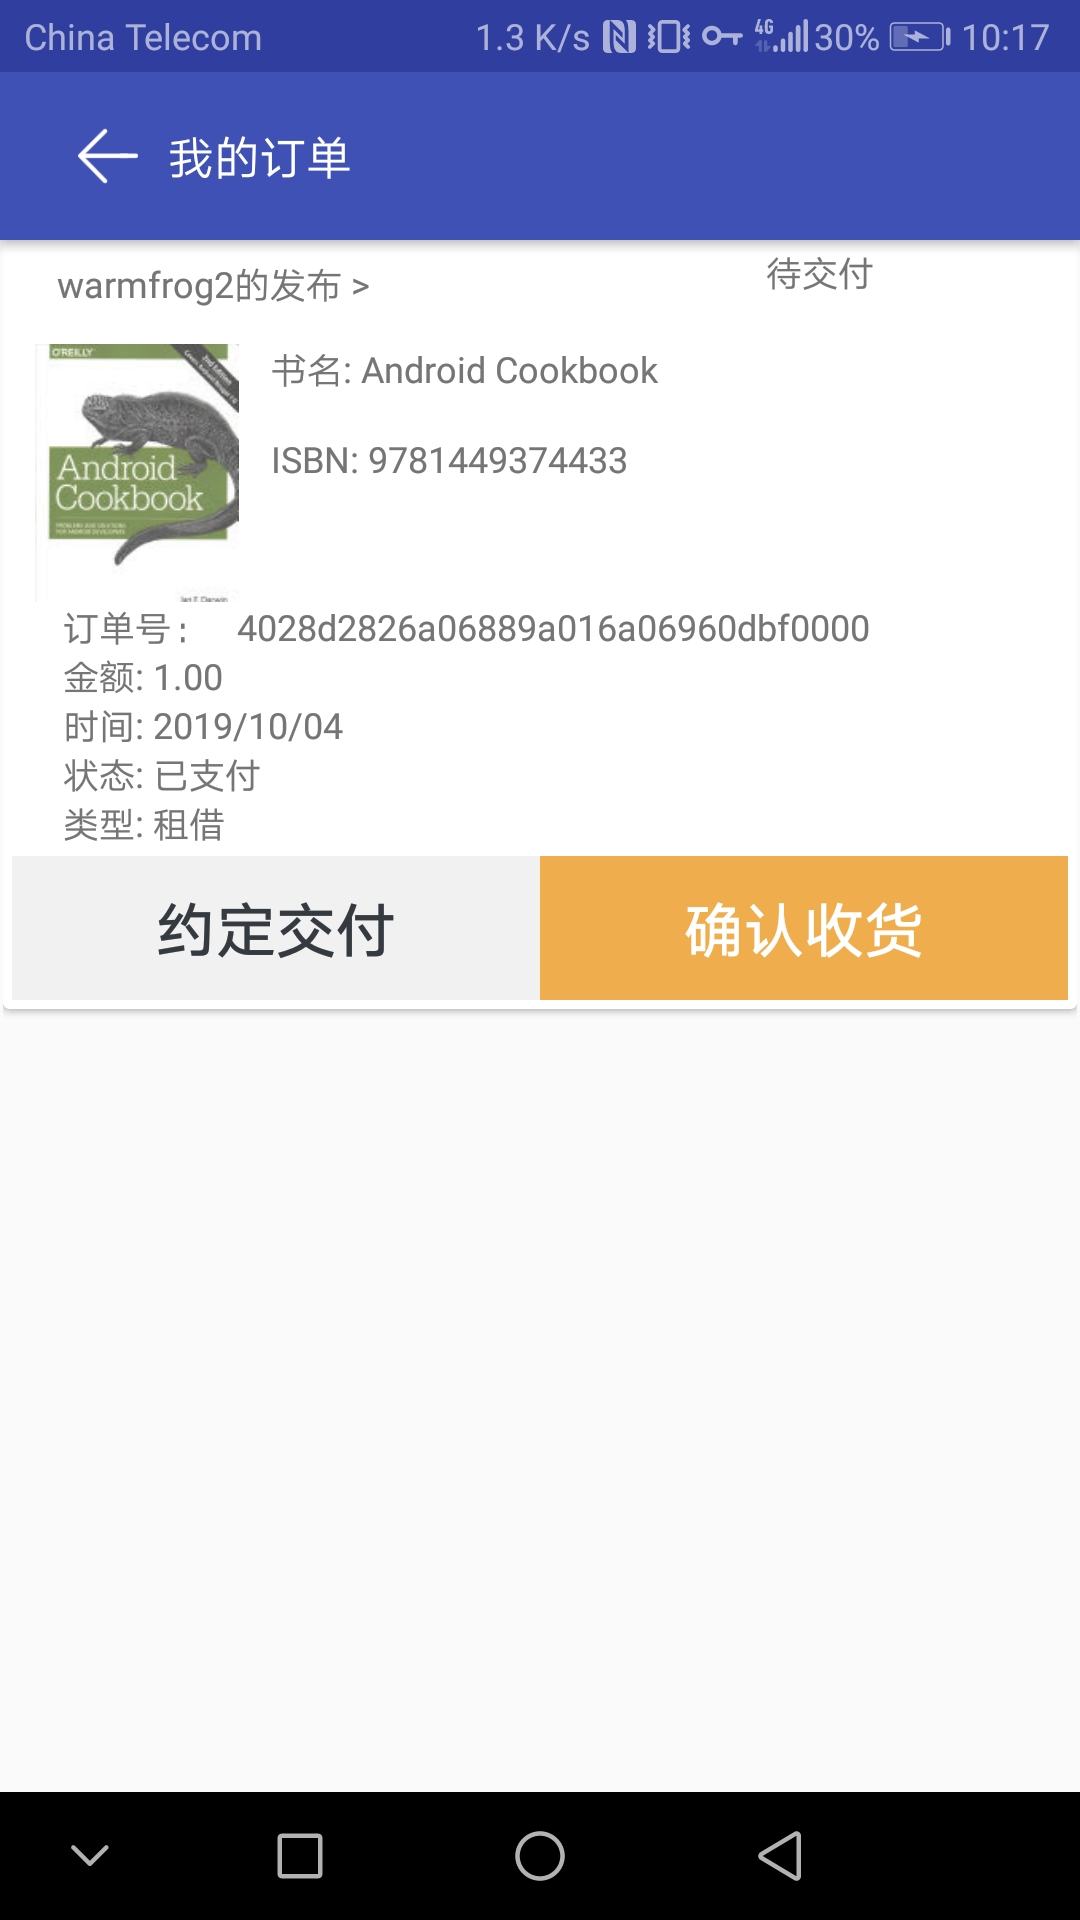
\includegraphics[scale=0.09]{Chapters/UI/unrecieved_order.jpg}
	\caption{我的订单}
	\label{unrecieved_order}
\end{figure}

订单包含了不同状态和类型。订单的类型包括租赁类型和购买类型。状态包括未支付状态,已支付状态,已完成状态和关闭状态。

用户下单时,租赁方式对应订单的租赁类型,购买对应订单的购买类型。用户下单后,订单为未支付状态,此时用户可以取消订单和支付订单。
用户支付订单后,订单变为已支付待交付状态,用户可以确认收获。消费者确认收货后,用户变成已完成状态,用户可以选择删除
订单信息。用户取消订单后,订单变为关闭状态,用户可以选择删除订单。

\cref{unrecieved_order}是我的订单页面。用户在个人主页点击我的订单时进入该页面。
显示用户所有的订单页面,用户可以对
订单进行状态的改变或者删除操作。



\subsection{钱包管理}
用户在下方的导航栏点击我的-我的钱包,进入我的钱包页面。我的钱包头部的动作栏包含一个返回按钮和标题余额。下方是提示信息余额账户
(书币),再下面是用户的账户余额,背景色为淡蓝色。下方是提示信息,提示用户如何获得书币。

目前书币获得策略设定为新注册用户获得两个书币,之后,用户每上传一部图书,都将获得一个书币。

\cref{balance}是我的钱包页面。当用户在个人主页点击个人钱包时进入该页面,该页面显示账户余额信息。

\begin{figure}[h]
	\centering
	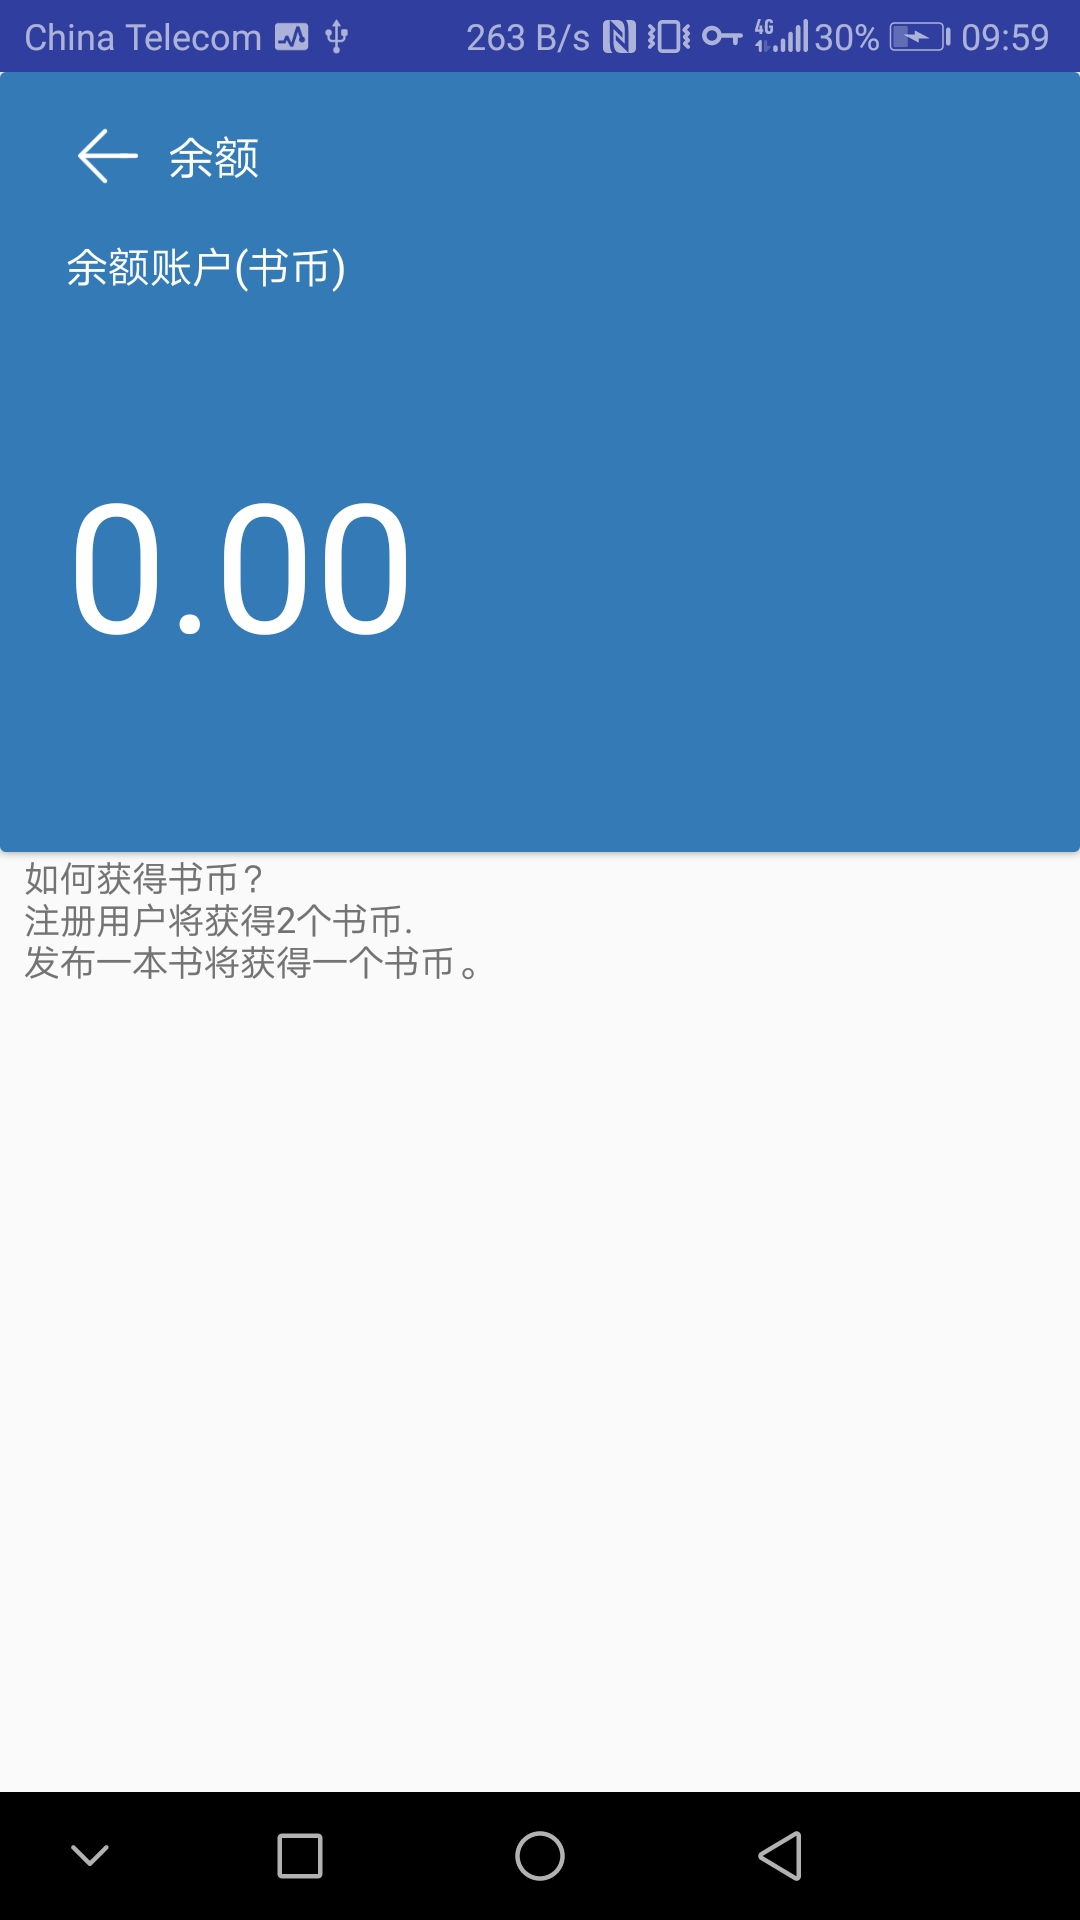
\includegraphics[scale=0.09]{Chapters/UI/balance.jpg}
	\caption{我的钱包}
	\label{balance}
\end{figure}

\subsection{清除缓存}
用户点击我的-清除缓存,将删除当前应用本地文件信息,用户属性信息,和本地 Sqlite 数据库所有数据。

\subsection{退出登录}
用户点击我的-退出登录,将删除用户本地属性文件中已登录的 token 信息。并进入默认的提示登录信息页面。之后,用户通过点击我的,只能
进入提示登录页面,用户只有登录后,才能进入个人主页。

\section{数据库设计}
		
\begin{enumerate}
	\item 用户表设计user
	
	\begin{table}[h]
		\centering
		\caption{用户表设计user}
		\label{user_table}
		\begin{tabular}{ccccc}
			\toprule
			\textbf{字段名} & \textbf{数据类型} & \textbf{长度} & \textbf{其他}  & \textbf{备注} \\
			\midrule
			id  & int & 11 & 主键 & 用户ID \\
			username & varchar & 255 & unique & 用户名 \\
			create\_date & datetime & default & not null & 用户创建时间 \\
			email & varchar & 255 & unique & 用户邮箱 \\
			enabled & bit & 1 &  & 用户是否有效 \\
			password & varchar & 255 & not null & 加密后的用户密码 \\
			phone & varchar & 255 & unique & 用户绑定手机 \\
			\bottomrule
		\end{tabular}
	\end{table}

	\cref{user_table}是用户表,用户表包含用户 ID,用户名,用户创建时间, 用户邮箱 , enabled ,用户密码,用户手机等字段。
	用户 ID 为数据库自增;用户名为 unique 类型,表示不能重复;用户邮箱和手机同样为 unique,不能重复;enabled 表示用户是否
	有效;用户密码保存加密过的用户密码。

	\item 图书表gbook\$volume\_info设计
	
	\cref{gbook$volume_info_table}是图书详情表,包含自增 ID,购买连接,内容版本,内容描述,详情连接,语言版本,
	成熟度评分,页数,预览链接,出版类型,出版日期,子标题,标题等字段。
	\begin{table}[h]
		\centering
		\caption{图书表Gbook设计}
		\label{gbook$volume_info_table}
		\begin{tabular}{ccccc}
			\toprule
			\textbf{字段名} & \textbf{数据类型} & \textbf{长度} & \textbf{其他}  & \textbf{备注} \\
			\midrule
			id  & int & 11 & 自增主键 & ubook ID \\
			allow\_anon\_logging & bit & 1 & not null & "" \\
			canonical\_volume\_link & varchar & 255 & null & 购买连接 \\
			content\_version & varchar &255 & null & 内容版本 \\
			description & varchar & 4096 & null & 内容描述 \\
			info\_link & varchar & 255 & null & 详情连接 \\
			language & varchar & 255 & null & 语言版本 \\
			maturity\_rating & varchar & 255 & null & 成熟度评分 \\
			page\_count & bigint & 20 & null & 页数 \\
			preview\_link & varchar & 255 & null & 预览链接 \\
			print\_type & varchar & 255 & null & 出版类型 \\
			published\_data & varchar & 255 & null & 出版日期 \\
			subtitle & varchar & 255 & null & 子标题 \\
			title & varchar & 255 & null & 标题 \\
			\bottomrule
		\end{tabular}
	\end{table}
	\item 发布图书表设计ubook
	
	\cref{ubook_table}是用户发布的图书字段,包含自增 ID,图书 ISBN,图书封面 url,图书简介,图书发布时间,租赁价格,出售价格,
	当前状态等字段。该表通过关联表 ubook-gbook 与具体图书信息关联。

	\begin{table}[h]
		\centering
		\caption{发布图书表设计ubook}
		\label{ubook_table}
		\begin{tabular}{ccccc}
			\toprule
			\textbf{字段名} & \textbf{数据类型} & \textbf{长度} & \textbf{其他}  & \textbf{备注} \\
			\midrule
			id  & int & 11 & 自增主键 & ubook ID \\
			isbn13 & varchar & 255 & unique & 图书13位的ISBN \\
			image & varchar & 255 & null & 图书图像url \\
			book\_intro & varchar & 255 & null & 图书简介 \\
			release\_time & datetime & default & not null & 图书发布时间 \\
			rent\_price & decimal & default & not null & 租赁价格 \\
			sell\_price & decimal & default & not null & 出售价格 \\
			status & varchar & 255 & not null & 当前状态 \\
			\bottomrule
		\end{tabular}
	\end{table}
	\item 订单表order设计
	
	\cref{order_table}是订单信息表,包含订单 ID,订单创建时间订单总额,订单状态,订单类型等字段。
	\begin{table}[h]
		\centering
		\caption{订单表order设计}
		\label{order_table}
		\begin{tabular}{ccccc}
			\toprule
			\textbf{字段名} & \textbf{数据类型} & \textbf{长度} & \textbf{其他}  & \textbf{备注} \\
			\midrule
			id  & varchar & 32 & UUID主键 & 订单ID \\
			create\_time & datetime & default & not null & 订单创建时间 \\
			price & decimal & default & not null & 订单总额 \\
			status & varchar & 255 & not null & 订单状态 \\
			type & int & 11 & not null & 订单类型(租赁,购买) \\
			\bottomrule
		\end{tabular}
	\end{table}
	\item 钱包表 wallet 设计
	
	\cref{wallet_table}包含 ID 和钱包余额等字段。
 	\begin{table}[h]
		\centering
		\caption{钱包表wallet设计}
		\label{wallet_table}
		\begin{tabular}{ccccc}
			\toprule
			\textbf{字段名} & \textbf{数据类型} & \textbf{长度} & \textbf{其他}  & \textbf{备注} \\
			\midrule
			id  & int & 11 & 自增主键 & 订单ID \\
			balance & decimal & default & not null & 钱包余额 \\
			\bottomrule
		\end{tabular}
	\end{table}
\end{enumerate}

\section{后端接口设计}
\subsection{用户相关接口/api/user/* 设计}

\cref{api_user}包含了后端用户 api 设计,对应地址前缀为"api/user/*"的地址,包含了与用户相关的 api。
包含了下列功能接口:添加用户,检查用户存在性,获取用户,更新用户,删除用户,发布图书,查询钱包余额,
下订单,取消订单,查看订单,支付订单,签收订单,删除订单。

\begin{table}[h]
	\centering
	\caption{用户相关接口/api/user/*}
	\label{api_user}
	\begin{tabular}{ccc}
		\toprule
		\textbf{映射} & \textbf{HTTP方法} & \textbf{用途} \\
		\midrule
		/ & GET & 获取用户列表  \\
		/ & POST & 添加用户 \\
		/check/\{username\} & GET &  检查用户是否存在 \\
		/\{id\} & GET & 获取用户相关信息 \\
		/\{id\} & PUT &  更新用户相关信息 \\
		/\{id\} & DELETE & 根据ID删除用户 \\
		/\{username\}/release & POST & 用户发布图书 \\
		/\{username\}/balance & GET & 查询用户余额 \\
		/\{username\}/order/\{ubookId\} & POST & 用户下单 \\
		/\{username\}/cancel/\{orderId\} & POST &  用户取消订单 \\
		/\{username\}/myorder & GET & 用户查看订单 \\
		/\{username\}/pay/\{orderId\} & POST & 用户支付订单 \\
		/\{username\}/sign/\{orderId\} & POST & 用户签收订单 \\
		/\{username\}/delete/\{orderId\} & DELETE & 用户删除订单 \\
			\bottomrule
	\end{tabular}
\end{table}

\subsection{发布书相关接口/api/ubook/* 设计}

\cref{api_ubook}包含了用户发布图书相关的 api 设计,包含的功能有获取图书信息,获取某个 ID 之前的发布
图书,获取某个 ID 之后的发布图书列表,获取前 10 本发布图书,删除发布图书

\begin{table}[h]
	\centering
	\caption{发布书相关接口/api/ubook/*}
	\label{api_ubook}
	\begin{tabular}{ccc}
		\toprule
		\textbf{映射} & \textbf{HTTP方法} & \textbf{用途} \\
		\midrule
		/ & POST & 发布图书 \\
		/\{username\}/count & GET & 用户发布图书数量 \\
		/\{id\} & GET & 根据ID获取图书信息 \\
		/\{id\}/before & GET & 获取ID之前的发布的图书 \\ 
		/\{id\}/after & GET & 获取ID之后的发布的图书 \\
		/top & GET & 获取前 10 本书 \\
		/\{id\} & DELETE & 根据ID删除发布的图书 \\
		/ & PUT & 更新发布图书 \\
			\bottomrule
	\end{tabular}
\end{table}

\subsection{gbook相关接口/api/gbook/* 设计}

\cref{api_gbook}包含了获取具体出版书的图书信息,功能包含获取具体图书信息,获取图片封面地址。

\begin{table}[h]
	\centering
	\caption{gbook相关接口/api/gbook/*}
	\label{api_gbook}
	\begin{tabular}{ccc}
		\toprule
		\textbf{映射} & \textbf{HTTP方法} & \textbf{用途} \\
		\midrule
		/isbn/\{isbn13\} & POST & 根据ISBN获取图书信息 \\
		/isbn/\{isbn13\}/image & GET & 根据ISBN获取图书封面地址 \\
			\bottomrule
	\end{tabular}
\end{table}




